\documentclass{article}
\usepackage{natbib}
\setcitestyle{numbers,square,comma}
\usepackage{multirow}

% if you need to pass options to natbib, use, e.g.:
% \PassOptionsToPackage{numbers, compress}{natbib}
% before loading neurips_2024


% ready for submission
% \usepackage{neurips_2024}
% \usepackage{etoolbox}
% \newtoggle{isSubmission}
% \toggletrue{isSubmission}

% camera ready for arxiv
\usepackage[preprint]{neurips_2025}
\usepackage{etoolbox}
\newtoggle{isSubmission}
\togglefalse{isSubmission}

% camera ready for submission
% \usepackage[final]{neurips_2024}
% \usepackage{etoolbox}
% \newtoggle{isSubmission}
% \toggletrue{isSubmission}

% to compile a preprint version, e.g., for submission to arXiv, add add the
% [preprint] option:
    % \usepackage[preprint]{neurips_2024}


% to compile a camera-ready version, add the [final] option, e.g.:
%     \usepackage[final]{neurips_2024}


% to avoid loading the natbib package, add option nonatbib:
%    \usepackage[nonatbib]{neurips_2024}

\usepackage{times}
\usepackage{epsfig}
\usepackage{graphicx}
\usepackage{amsmath}
\usepackage{amssymb}


% \usepackage{subfigure}
\usepackage{booktabs} 
\usepackage{diagbox}
\usepackage{multirow}
\usepackage{ifthen}
\usepackage{lineno}
\usepackage{ifthen}
\usepackage{cases}
\usepackage{footnote}
\usepackage{lipsum}
\makesavenoteenv{table}
\usepackage{array}
\usepackage{makecell} % 用于在单元格中换行
\usepackage{tabularx} % 用于自动调整列宽
% \usepackage{pifont}       % \ding{xx}
\usepackage{bbding}       % \Checkmark,\XSolid,... (需要和pifont宏包共同使用)
\usepackage{fontawesome}  % \faCheck,\faTimes

% to compile a preprint version, e.g., for submission to arXiv, add add the
% [preprint] option:
%     \usepackage[preprint]{neurips_2025}


% to compile a camera-ready version, add the [final] option, e.g.:
%     \usepackage[final]{neurips_2025}


% to avoid loading the natbib package, add option nonatbib:
%    \usepackage[nonatbib]{neurips_2025}
\usepackage{hyperref}       % hyperlinks
\hypersetup{
    colorlinks,
    linkcolor={red!85!black},
    citecolor={blue!70!cyan},
    urlcolor={blue!90!black}
}

\usepackage[utf8]{inputenc} % allow utf-8 input
\usepackage[T1]{fontenc}    % use 8-bit T1 fonts
\usepackage{url}            % simple URL typesetting
\usepackage{booktabs}       % professional-quality tables
\usepackage{amsfonts}       % blackboard math symbols
\usepackage{nicefrac}       % compact symbols for 1/2, etc.
\usepackage{microtype}      % microtypography

\usepackage{xspace}
\newcommand{\ie}{\textit{i.e.}\xspace}
\newcommand{\eg}{\textit{e.g.}\xspace}
\newcommand{\etal}{\textit{et al.}\xspace}
\newcommand{\etc}{\textit{etc.}\xspace}

\newcommand*{\affaddr}[1]{#1} 
\newcommand*{\affmark}[1][*]{\textsuperscript{#1}}
\newcommand{\authormark}[2][]{%
  \begingroup
  \def\@thefnmark{#1}%
  \footnote{#2}%
  \endgroup
}


\title{VCapsBench: A Large-scale Fine-grained Benchmark for Video Caption Quality Evaluation}


% The \author macro works with any number of authors. There are two commands
% used to separate the names and addresses of multiple authors: \And and \AND.
%
% Using \And between authors leaves it to LaTeX to determine where to break the
% lines. Using \AND forces a line break at that point. So, if LaTeX puts 3 of 4
% authors names on the first line, and the last on the second line, try using
% \AND instead of \And before the third author name.
% Shi-Xue Zhang
% ~Shi-Xue_Zhang1
% , Hongfa Wang, Duojun Huang, Xin Li, Xiaobin Zhu, Xu-Cheng Yin
\author{%
\bf
Shi-Xue Zhang \affmark[1,2]\thanks{Equal contribution}~~
Hongfa Wang\affmark[2,3]\textsuperscript{*}~~
Duojun Huang\affmark[2]\textsuperscript{*}~~ 
Xin Li\affmark[2]\textsuperscript{*}\\
\bf
Xiaobin Zhu\affmark[1]\textsuperscript{$^\dagger$}~~ 
Xu-Cheng Yin\affmark[1]\thanks{Corresponding author}~~~ \\
\affaddr{\affmark[1]University of Science and Technology Beijing}
\affaddr{\affmark[2]Tencent} \\
\affaddr{\affmark[3]Tsinghua Shenzhen
International Graduate School}
}

% customized packages and commands
\bibliographystyle{unsrt}
\usepackage{graphics}
\usepackage[table]{xcolor}
\usepackage{subcaption}
\usepackage{caption}
\usepackage{amssymb}
\usepackage{algorithm}
\usepackage{algpseudocode}
\usepackage{wrapfig}
\usepackage{longtable}
\usepackage{fancyvrb}
\usepackage{empheq}
\definecolor{metacolor}{HTML}{0064E0}
\hypersetup{
  colorlinks,
  linkcolor=metacolor,
  citecolor=metacolor,
  urlcolor=metacolor
}
\usepackage{adjustbox}
\usepackage{makecell} 
\definecolor{color_blue}{HTML}{E7EFFA}
\definecolor{color_green}{HTML}{E6F8E0}
\definecolor{color_gray}{HTML}{ECECEC}
\definecolor{pearDark}{HTML}{2980B9}



\begin{document}


\maketitle
\begin{abstract}
Video captions play a crucial role in text-to-video generation tasks, as their quality directly influences the semantic coherence and visual fidelity of the generated videos. Although large vision-language models (VLMs) have demonstrated significant potential in caption generation, existing benchmarks inadequately address fine-grained evaluation, particularly in capturing spatial-temporal details critical for video generation. To address this gap, we introduce the Fine-grained Video Caption Evaluation Benchmark (\textbf{VCapsBench}), the first large-scale fine-grained benchmark comprising 5,677 (5K+) videos and 109,796 (100K+) question-answer pairs. These QA-pairs are systematically annotated across 21 fine-grained dimensions (\eg, camera movement, and shot type) that are empirically proven critical for text-to-video generation. We further introduce three metrics (Accuracy (\textbf{AR}), Inconsistency Rate (\textbf{IR}), Coverage Rate (\textbf{CR})), and an automated evaluation pipeline leveraging large language model (LLM) to verify caption quality via contrastive QA-pairs analysis. By providing actionable insights for caption optimization, our benchmark can advance the development of robust text-to-video models. The dataset and codes are available at website: \url{https://github.com/GXYM/VCapsBench}. 
\end{abstract}

\begin{figure}[ht]
	\begin{minipage}[t]{1.0\linewidth}
        \centering
	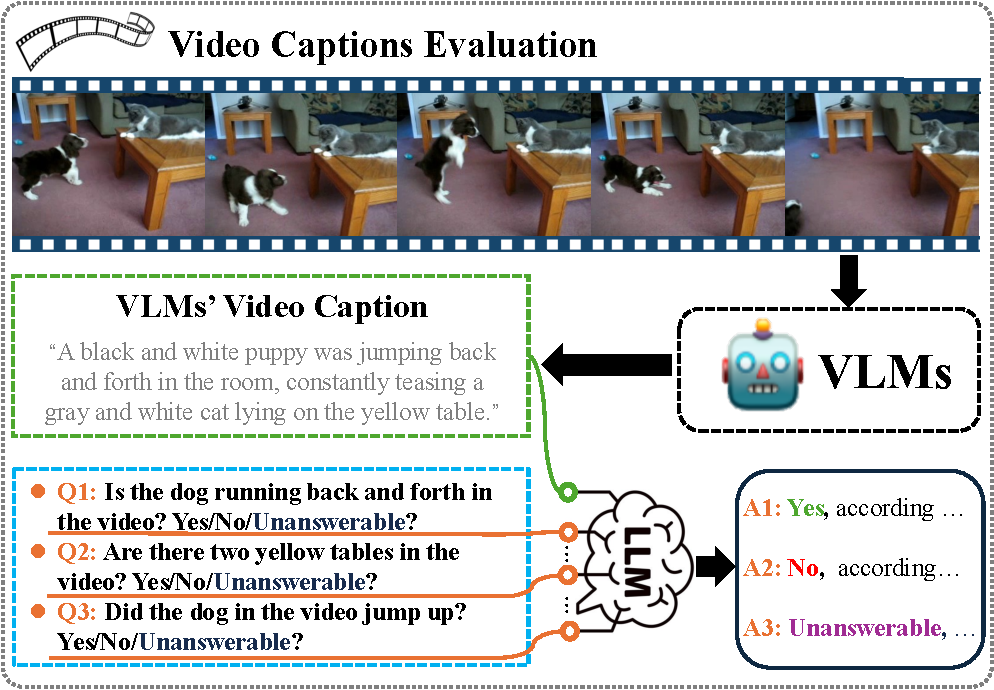
\includegraphics[width=0.8\linewidth]{imgs/intro-2.pdf}
	\caption{Illustration of video caption evaluation by VCapsBench. Evaluate the detail, comprehensiveness, and accuracy of video captions using "yes-no" question-answer pairs.}
	\label{fig:fig1}
	\end{minipage}%
	\vspace{-1.5em}	
\end{figure}    
\section{Introduction}
\label{sec:intro}
Recent advances in video understanding~\cite{reid2024gemini, liu2025st, hong2024cogvlm2, liu2024oryx, zhang2024STGT, li2024aria} and generation~\cite{SORA, vidu, kelin, hunyuanvideo} have been driven by large vision-language models (VLMs). For video comprehension, researchers have extended image-based architectures (\eg, LLaVA-Video~\cite{zhang2024video}, PLLaVA~\cite{xu2024pllava} and CogVLM2-Video~\cite{hong2024cogvlm2}) and explored hybrid image-video training approaches (Qwen2-VL~\cite{wang2024qwen2}, LLaVA-OneVision~\cite{li2024llava}). Currently, video generation systems such as Sora~\cite{SORA} and HunyuanVideo~\cite{hunyuanvideo} use VLMs for multimodal captioning and prompt engineering. However, current benchmarks~\cite{li2024mvbench, li2024videovista, wang2024lvbench, fu2024video, zhou2024mlvu, wu2024longvideobench} struggle to assess the detailed spatio-temporal aspects required for these applications.


In visual generation, existing caption evaluation metrics fall mainly into two categories: reference-based (METEOR~\cite{meteor}, BLEU~\cite{bleu}, SPICE~\cite{Spice}, and CIDEr~\cite{cider}) and reference-free (InfoMetIC~\cite{infometic}, CLIPScore~\cite{Clipscore}, and TIGEr~\cite{Tiger}). Reference-based metrics~\cite{meteor,bleu,Spice,cider} assess the quality of the captions by comparing them with ground-truth captions. However, these scores are highly dependent on the reference captions' format. Hence, FAIEr~\cite{Faier} adopts visual and textual scene graphs for a more robust reference-based evaluation. Reference-free metrics~\cite{infometic,Clipscore,Tiger} use semantic vectors from the reference image to evaluate the similarity of the caption. These methods falter with concept-dense captions, overwhelmed by numerous concepts. Recent innovations like QACE~\cite{QACE}, DSG ~\cite{cho2023davidsonian}], DPG-bench~\cite{Ella} and CapsBench~\cite{playgroundv3} employ question-answering frameworks to address dense concept evaluation for image captioning. Notably, these methods derived from image description evaluation still have significant measurement blind spots when dealing with the spatio-temporal dynamic elements of video generation scenarios, \eg,  camera motion (``slow zoom" vs. ``fast pan") or dynamic spatial relationships (object displacement from ``left foreground " to ``central midground"). 
In these cases, video generation systems (\eg, Sora) need to ensure accurate text-video alignment.

Current video understanding benchmarks primarily focus on holistic semantic alignment (MVBench ~\cite{li2024mvbench}, VideoVista~\cite{li2024videovista}) or specific skill evaluation (LVBench~\cite{wang2024lvbench}), neglecting fine-grained spatial-temporal dynamics essential for video generation. This gap becomes critical when evaluating text-to-video systems where caption precision directly impacts visual output. For instance, failing to distinguish between ``slow zoom" versus ``fast pan" camera motions, or misrepresenting object trajectories from ``left foreground" to ``central midground". While manual evaluation of such nuances remains impractical at scale, automated metrics also struggle with dynamic semantic alignment due to inherent limitations in traditional evaluation paradigms. To address this problem, it is necessary to re-examine the design principles of video description evaluation metrics.

To address critical gaps in evaluating video caption,  we introduce \textbf{VCapsBench}, the first large-scale fine-grained benchmark for video caption evaluation. It contains 5,677 diverse videos with 109,796 human-verified questions, allowing fine-grained evaluation of caption quality. Specifically, we employ text-based question-answering across 21 categories, including action, camera movements (\eg, zoom, pan and tilt), object positioning (absolute or relative position), entity and shot type, \etc, with ``yes", ``no", and ``unanswerable" ternary judgments. Unlike image-focused caption benchmarks like CapsBench~\cite{playgroundv3}, our VCapsBench prioritizes temporal continuity through video-specific queries (avg. 19 questions/video) while mitigating LLM hallucination via an ``Unanswerable" option. To accurately and comprehensively assess caption quality, we introduce three metrics: Accuracy (AR), Inconsistency Rate (IR), and Coverage Rate (CR). To automate the calculation of these metrics, we develop an evaluation pipeline that leverages powerful LLMs for objective video caption quality measurement, as illustrated in Fig.~\ref{fig:fig1}. In summary, our contributions are as follows:
\begin{itemize}
    \item We introduce \textbf{VCapsBench}, the first large-scale fine-grained benchmark for video caption evaluation, featuring diverse videos (5K+) and QA-pairs (100K+).
    \item We introduce three metrics: Accuracy (\textbf{AR}), Inconsistency Rate (\textbf{IR}), and Coverage Rate (\textbf{CR}), along with an automated evaluation pipeline to fairly assess the correctness and coverage of video captions.
    
    \item We evaluate ten VLMs, including seven advanced open models (Qwen2VL, Qwen2.5VL, InternVL2.5, LLaVA-Video, and VideoLLaMA3, \etc) and three closed model, GPT-4o,  Gemini2.5-Pro Flash and Preview, providing a solid reference for the community.
\end{itemize}






\section{Related Work}
\label{sec:RelatedWork}

\textbf{Reference-based metric methods}~\cite{meteor, bleu, Spice, cider, Faier} evaluate caption quality by comparing generated captions with ground-truth captions. BLEU~\cite{bleu} is a fast, cost-effective, and language-independent metric for machine translation, correlating well with human assessments. METEOR~\cite{meteor} also evaluates machine translation and shows a high correlation with human judgments, significantly outperforming BLEU. CIDEr~\cite{cider} measures the similarity of generated sentences against a set of human-written ground-truth sentences, serving as an automatic consensus metric for image description quality. However, these metrics primarily focus on n-gram overlap, which is neither necessary nor sufficient for simulating human judgment. To address these limitations, SPICE introduces a metric based on semantic propositional content over scene graphs, though its scores highly rely on the format of reference captions.  Newer methods like FAIEr~\cite{Faier} leverage visual and textual scene graphs for a more robust evaluation.

\textbf{Reference-free metric methods}~\cite{infometic, Clipscore, Tiger} utilize semantic vectors from the reference image to assess caption similarity. InfoMetIC~\cite{infometic} is an informative metric for reference-free image caption evaluation, capable of identifying incorrect words and unmentioned image regions with fine-grained precision. It provides a text precision score, a vision recall score, and an overall quality score at a coarse-grained level, with the latter showing significantly better correlation with human judgments than existing metrics across multiple benchmarks. CLIPScore~\cite{Clipscore} employs CLIP~\cite{clip} for robust automatic evaluation of image captioning without references, focusing on image-text compatibility. Although complementary to reference-based metrics that emphasize text-text similarities, CLIPScore is relatively weaker for tasks requiring richer contextual knowledge, such as news captions. TIGEr~\cite{Tiger} assesses caption quality by evaluating both the representation of image content and the alignment of machine-generated captions with human-generated ones.


\textbf{Question-based evaluation methods}~\cite{QACE, cho2023davidsonian, playgroundv3} have been developed to enhance the assessment of caption quality in visual generation tasks. The QACE framework~\cite{QACE} generates questions from captions to evaluate their quality. A similar approach has been proposed for image generation models, where the Davidsonian Scene Graph (DSG)~\cite{cho2023davidsonian} organizes questions into dependency graphs, facilitating comprehensive evaluation of text-to-image models. Inspired by DSG and DPG-bench~\cite{Ella}, Playground v3~\cite{playgroundv3} introduces CapsBench, a benchmark for image captioning that uses ``yes-no" question-answer pairs. However, these benchmarks focus solely on image captioning, while video captioning requires consideration of additional factors such as actions, motion, camera movements, and shot types, which are crucial for text-to-video generation.
\section{The VCapsBench Benchmark}


\subsection{Overview}
Although existing benchmarks can assess the quality of VLM-generated image captions across various dimensions, as discussed in Sec.~\ref{sec:RelatedWork}, they still fall short in evaluating the fine-grained video captions produced by VLMs. To effectively measure the understanding and descriptive capabilities of VLMs across different types of video, we have constructed a large-scale high-quality benchmark VCapsBench for video caption quality evaluation.

\begin{figure*}[tp]
	\begin{minipage}[t]{1.0\linewidth}
        \centering
	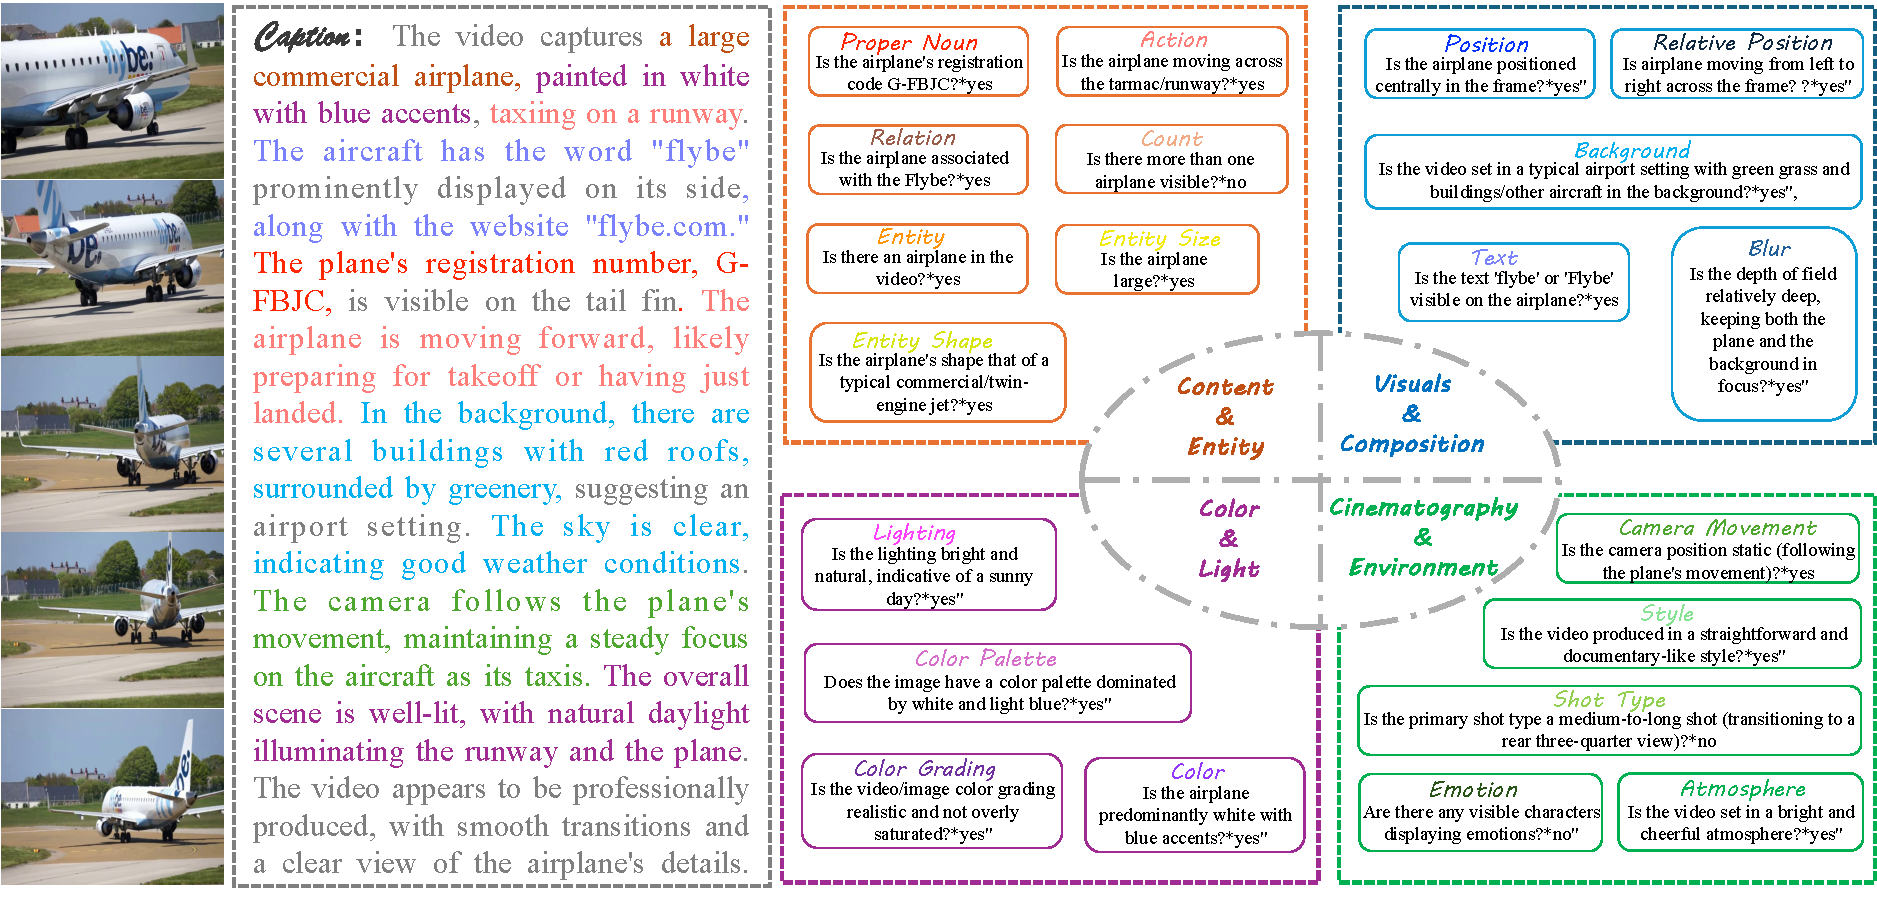
\includegraphics[width=0.95\linewidth]{imgs/method1-3.pdf}
	\caption{An example of video caption and  question-answer pairs in our VCapsBench.}
	\label{fig:fig2}
	\end{minipage}%
	\vspace{-1.0em}	
\end{figure*}

\begin{figure*}[tp]
	\begin{minipage}[t]{1.0\linewidth}
        \centering
	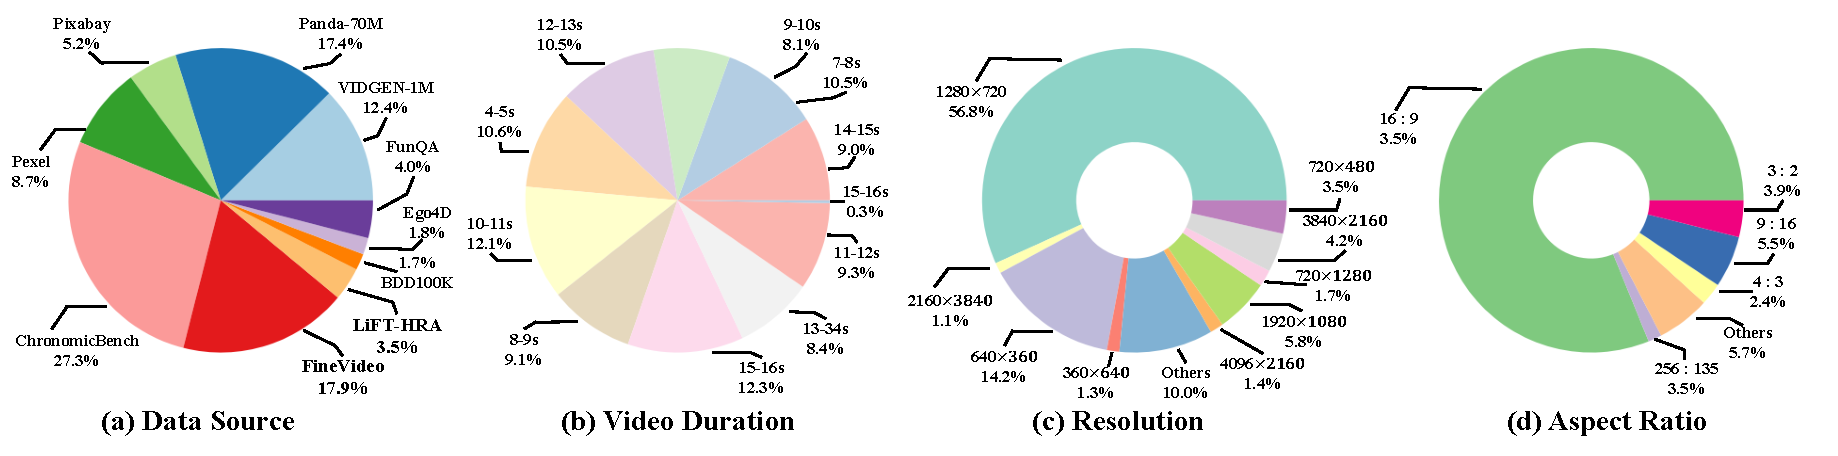
\includegraphics[width=0.95\linewidth]{imgs/method3-3.pdf}
	\caption{(a) Video source distribution; (b) Video duration distribution; (c) Video resolution distribution (d) Video aspect ratio distribution.}
	\label{fig:fig3}
	\end{minipage}%
	\vspace{-1.5em}	
\end{figure*}


\subsection{Dataset Statistics}
\textbf{Data Dimensions.} As shown in Fig.~\ref{fig:fig2}, the evaluation of video captions is organized into four primary categories: ``Content and Entity", ``Visuals and Composition" ``Color and Lighting" and ``Cinematography and Atmosphere". ``Content and Entity" includes seven subcategories, which focus on core elements like action, count, entity, entity size, entity shape, proper noun and relation. ``Visuals and Composition" is related to spatial arrangement and visual presentation, comprising five subcategories: position, relative position, text, blur, and background. ``Color and Lighting" addresses how these elements enhance mood and style, covering four subcategories: color, color palette, color grading, and lighting. Finally, ``Cinematography and Atmosphere" includes five subcategories: camera movement, shot type, style, atmosphere, and emotion, integrating filming techniques and artistic expression.  By categorizing these dimensions, it becomes easier to statistically analyze the quality of video  captions across different categories. This provides more detailed guidance for optimizing VLM's video understanding capabilities.

\textbf{Data Collection.} To fully support the caption evaluation task in video understanding and generation tasks, we prioritized  the complexity of aesthetic and content in our data collection for VCapsBench. We sourced videos from 10 publicly available datasets to ensure diversity: Panda-70M\cite{ChenSMDCJF0RYT24}, Ego4D\cite{grauman2022ego4d}, BDD100K\cite{yu2020bdd100k}, Pixabay~\cite{chensharegpt4video}, Pexel~\cite{chensharegpt4video}, VIDGEN-1M\cite{tan2024vidgen}, ChronomicBench~\cite{yuan2024chronomagic}, FineVideo~\cite{Farre2024FineVideo}, FunQA~\cite{yuan2024chronomagic}, and LiFT-HRA-20K~\cite{wang2024lift}. As illustrated in Fig.~\ref{fig:fig3}, we curated a diverse collection of 988 high-resolution videos from Panda-70M\cite{ChenSMDCJF0RYT24}, encompassing a wide range of scenes such as wildlife, cooking, sports, TV shows, gaming, and 3D rendering. These videos often contain complex content and transformations, providing a robust foundation for understanding various real-world scenarios. Additionally, we included 494 high-resolution videos from Pexels and 298 from Pixabay, both renowned for their scenic landscapes and human activities, characterized by high aesthetic quality and detailed imagery. To further ensure data diversity, we sample 1,018 videos from FineVideo\cite{Farre2024FineVideo}, which encompasses 6 major categories and 122 subcategories. Despite their lower resolution (below 640 $ \times $360), we balanced this by sampling 333 ultra-high-resolution videos (2K, 3K, and 4K) from VIDGEN-1M\cite{tan2024vidgen}, typically used for training text-to-video models due to their high detail and quality. Our collection was further enriched with videos from Ego4D\cite{grauman2022ego4d} and BDD100K\cite{yu2020bdd100k} to cover ego-centric human activities and autonomous driving scenarios, ensuring a comprehensive representation of real-world scenes.
To evaluate the VLM model's understanding of object motion and physical laws, we included 1,549 videos from ChronomicBench, spanning four main categories
(\eg, biological, artificial, meteorological, and physical) across 75 subcategories. To further diversify our dataset, we sampled 227 videos from FunQA and 200 from LiFT-HRA-20K. FunQA features human-centric content such as humorous clips, creative performances, and visual illusions, while LiFT-HRA-20K consists of synthetic video data.


As shown in Fig.~\ref{fig:fig3}, our VCapsBench dataset comprises 5,677 videos from a wide range of scenes, e.g., natural landscapes, animals, human activities, physical phenomena, games, 3D renderings, and synthetic videos (more than 100 subcategories). VCapsBench also features diverse video durations (4 to 16 seconds), resolutions (125 different resolutions), and aspect ratios (87 different ratios). This extensive collection allows for a thorough evaluation of VLM models' understanding and insight across various video types, ensuring a robust assessment of video captioning.

\begin{figure*}[thbp]
	\begin{minipage}[t]{1.0\linewidth}
        \centering
	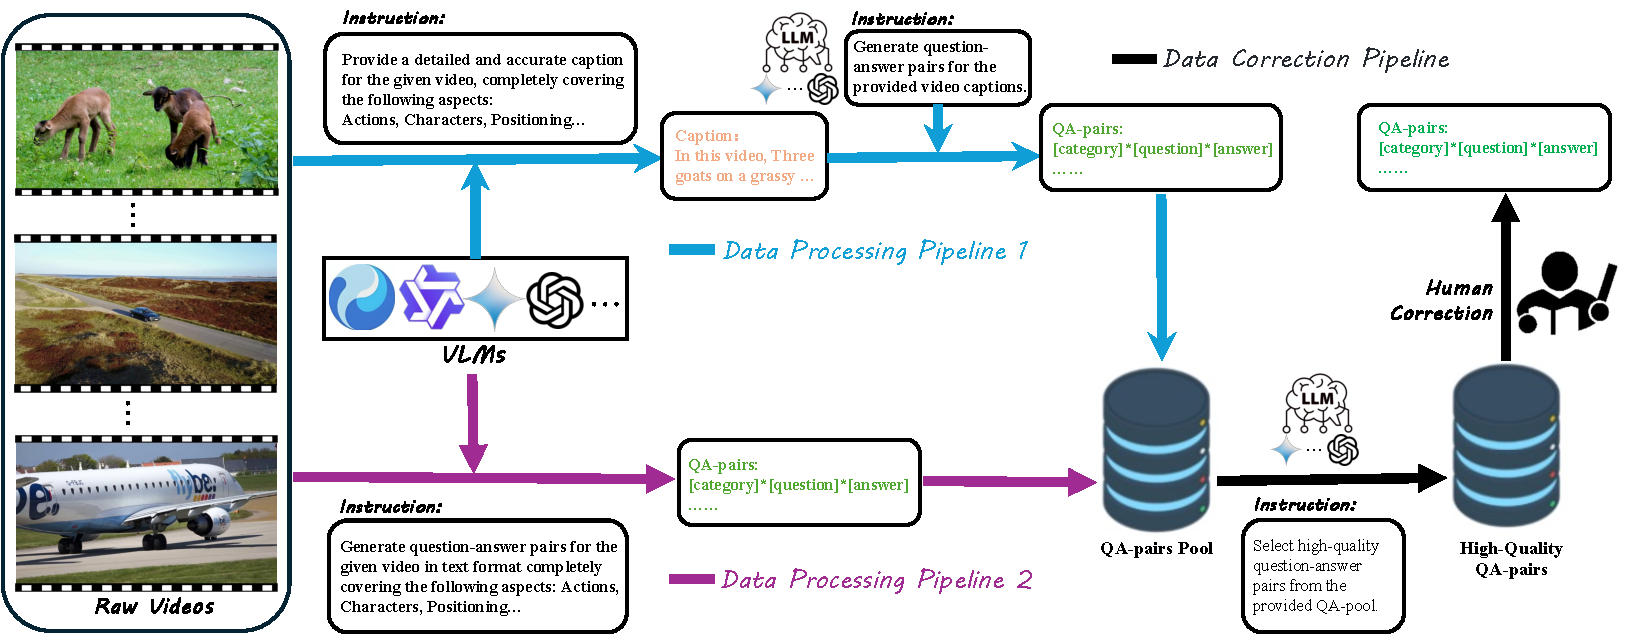
\includegraphics[width=0.9\linewidth]{imgs/method2.pdf}
	\caption{The pipeline of QA-pairs generation, which includes multiple data processing pipelines and a data correction pipeline.}
	\label{fig:fig4}
	\end{minipage}%
	\vspace{-1.0em}	
\end{figure*}

\subsection{Annotation Details}
Inspired by DPG-bench~\cite{Ella} and CapsBench~\cite{playgroundv3}, we developed a method to evaluate video caption quality using multi-dimensional question-answer pairs. Based on the raw video, we generate ``yes-no" question-answer pairs as annotations. As shown in Fig.~\ref{fig:fig4}, our ``Data Processing Pipeline" creates these pairs, which are stored in the ``QA-pairs Pool". Each pair includes a category, question, and answer, formatted as ``[category][question][answer]" for easy processing. To ensure diversity and accuracy, we designed two data production pipelines. The first one uses various VLMs, such as Geinimi, Qwen, and HunYuan, to generate detailed video captions from predefined prompts. Large Language Models (LLMs) like GPT-4, Gemini, and Qwen72B then use these captions and additional prompts to create question-answer pairs. The second approach directly utilizes VLMs to generate question-answer pairs from videos and prompts. The outputs from both pipelines are then combined into a comprehensive question-answer pool.


\begin{figure}[tp]
	\begin{minipage}[t]{1.0\linewidth}%\centering
	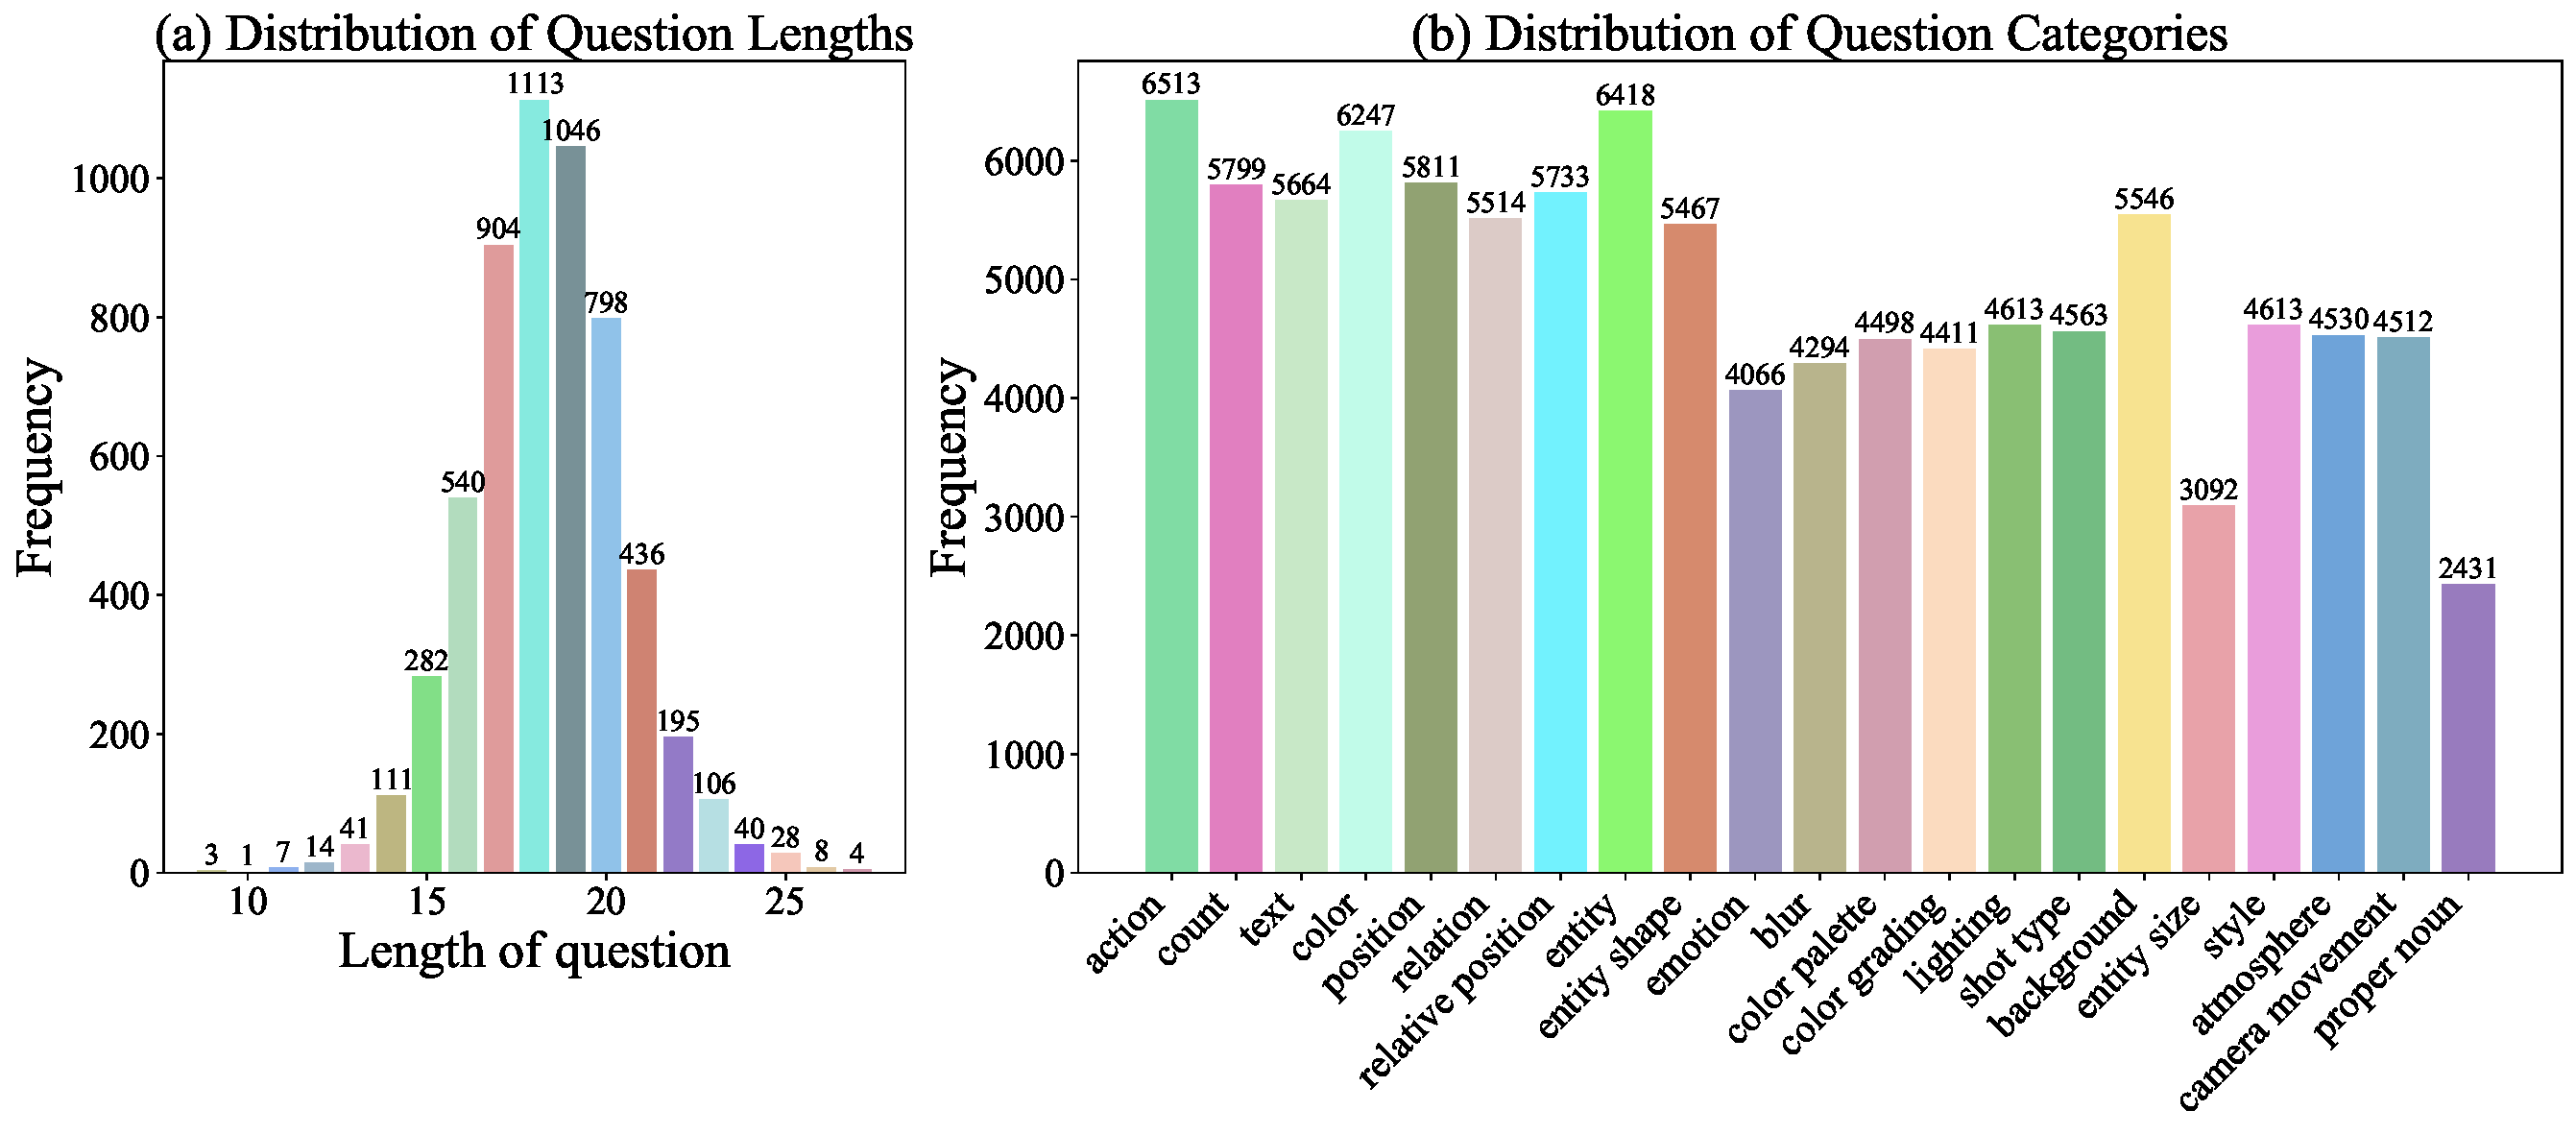
\includegraphics[width=0.9\linewidth]{imgs/qa_distribution-2.pdf}
	\caption{The question length and category distribution.}
	\label{fig:fig5}
	\end{minipage}%
	\vspace{-1.0em}	
\end{figure}

To enhance the quality of the QA-pairs, we established a data correction pipeline. This pipeline takes multiple sets of QA-pairs and captions from the same video as input and uses an advanced LLM (Gemini1.5) with predefined instructions to de-duplicate, filter, and retain high-quality QA-pairs. The instructions guide the LLM to merge similar QA-pairs, filter out those with the same question but different answers, and remove QA-pairs that appear only once, as they are likely to be invalid.



\textbf{Human Correction.} After generating high-quality candidate QA-pairs, we sample the data according to latitude to ensure that the data focuses more on important latitudes, and then conduct a final quality control process manually. Human reviewers re-examine these QA-pairs, deleting those with unreasonable or incorrect questions and correcting those with erroneous answers. Following this manual revision, we establish a benchmark (VCapsBench) consisting of 5,677 videos and 109,796 question-answer pairs. As shown in Fig.~\ref{fig:fig5}, each video contains between 10 and 27 QA-pairs, with each category comprising between 2,431 and 6,513 QA-pairs. The questions are organized into four major categories and 21 subcategories. Most answers are ``yes" providing a clear indication of correctness, while a smaller number of ``no" answers help assess whether the video captions contain hallucinations or inaccuracies.


\begin{figure*}[tp]
	\begin{minipage}[t]{1.0\linewidth}
        \centering
	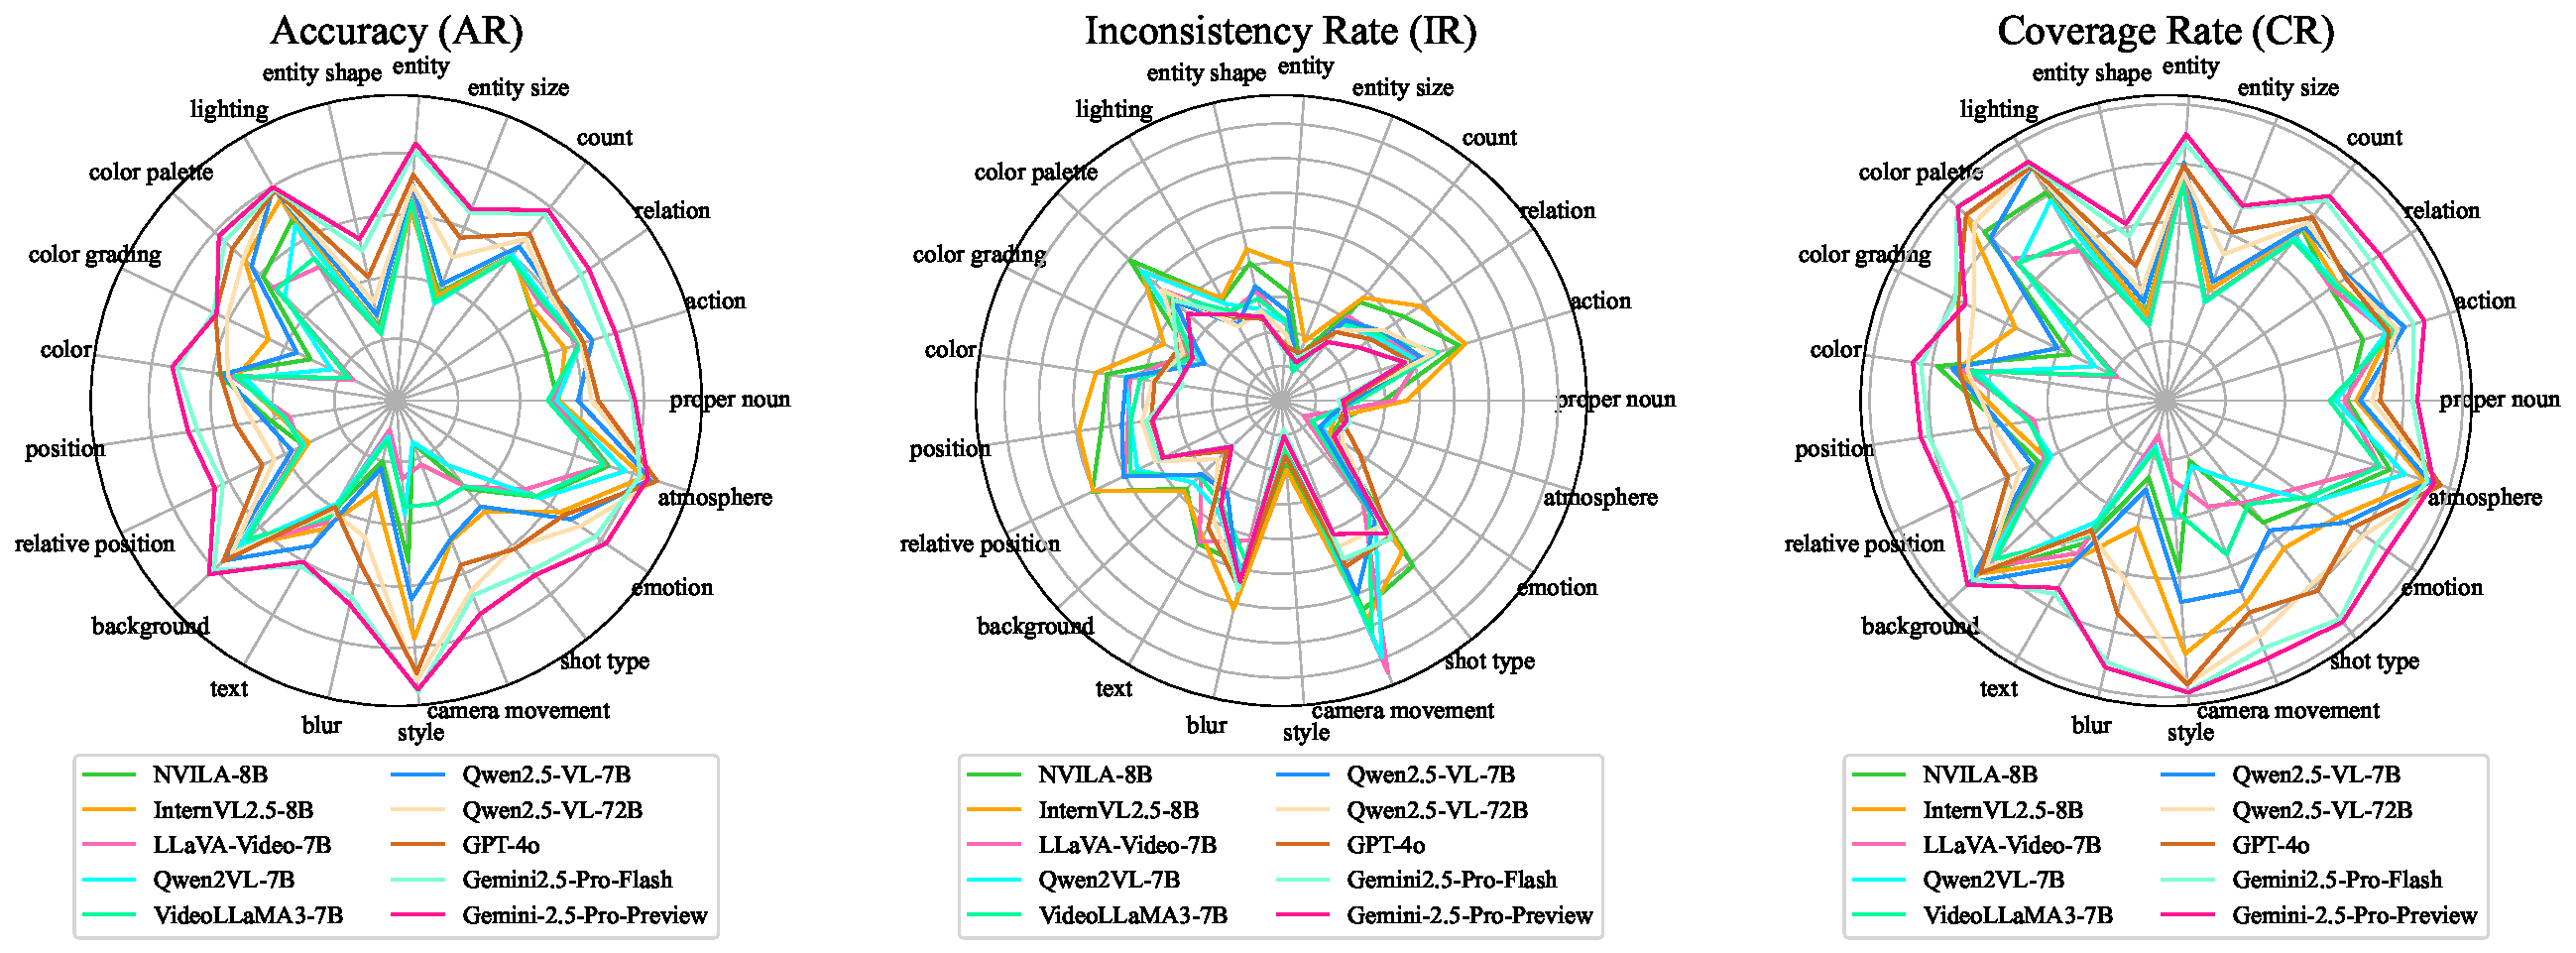
\includegraphics[width=1.0\linewidth]{imgs/radar_chart_all-New.pdf}
	\caption{Results of Gemini-2.5-Pro-Preview captioning evaluation, organized by category.}
	\label{fig:fig6}
	\end{minipage}%
	\vspace{-1.5em}	
\end{figure*}

\subsection{Captioning Evaluation}
We employ VCapsBench to evaluate video captions produced by various vision-language models (VLMs), including top proprietary models like Gemini-1.5. For each test video, an evaluation-capable VLM generates a detailed caption according to specific guidelines and an output schema. This caption, along with each question from the video's QA pairs, is fed into a Large Language Model (LLM). As shown in Fig.~\ref{fig:fig1}, the LLM responds to each question based on the caption, providing answers in the format ``[answer], [reason]." We instruct the LLMs to assess the caption in the following three scenarios:

\begin{itemize}
    \item \textbf{Positive:} The caption accurately describes the relevant content, and the LLM's response aligns with the answer.
    
    \item \textbf{Negative:} The caption mentions the relevant content, but the LLM's response does not align with the answer.
    
    \item \textbf{Unanswerable:} The caption does not involve the relevant content for the dimension.
\end{itemize}

To comprehensively evaluate the quality of the captions, we developed three metrics tailored to these scenarios. The quality of the captions is evaluated using the following measure:

\begin{equation}
AR = \dfrac{N(\text{Positive})}{N(\text{All})},
\end{equation}

\begin{equation}
IR = \dfrac{N(\text{Negative})}{N(\text{Positive}) + N(\text{Negative})},
\end{equation}

\begin{equation}
CR = \dfrac{N(\text{Positive}) + N(\text{Negative})}{N(\text{All})},
\end{equation}


\textbf{Accuracy (AR):} This metric evaluates the percentage of ``Positive" responses, indicating that the caption correctly describes the relevant content and aligns with the LLM's response. A higher AR signifies a more accurate and reliable caption, reflecting better quality in the LLM's outputs.

\textbf{Inconsistency Rate (IR):} This metric measures the percentage of ``Negative" responses among all responses that reference the relevant content (both ``Positive" and ``Negative"). A lower IR denotes a more accurate caption, indicating that when the caption involves relevant content, it is more likely to be consistent with the real video content.

\textbf{Coverage Rate (CR):} This metric evaluates the total percentage of "Positive" and ``Negative" responses, reflecting whether the caption contains the relevant content, independent of the LLM's response consistency. A higher CR indicates a superior caption richness, as it suggests that the caption encompasses a greater amount of pertinent content from the video.


\begin{table*}[!t]
\renewcommand{\arraystretch}{0.6}
\caption{The accuracy (AR), inconsistency rate (IR), and coverage rate (CR) of VLM methods on all dimensions, where Gemini-2.5-Pro-Preview as a TextQA expert. The symbol ``$\uparrow$"  indicates that the larger the value, the better; The symbol ``$\downarrow$" indicates that the smaller the value, the better.}
\label{tab:results_1}
\resizebox{\textwidth}{!}{%
\begin{tabular}{@{}ll|cccccccccccc@{}}
\toprule
 &\multirow{3}{*}{Methods}& \multicolumn{7}{c|}{Content \& Entity}& \multicolumn{4}{c}{Color \&  Light}\\
 \cline{3-13} 
 &  & \begin{tabular}[c]{@{}c@{}}\small Proper\\ \small Noun\end{tabular} & \begin{tabular}[c]{@{}c@{}}Action\end{tabular} & \begin{tabular}[c]{@{}c@{}}Relation
\end{tabular} & \begin{tabular}[c]{@{}c@{}}Count
\end{tabular} & Entity  & \begin{tabular}[c]{@{}c@{}}\small Entity\\ \small Size\end{tabular} & \multicolumn{1}{c|}{\begin{tabular}[c]{@{}c@{}}\small Entity\\ \small Shape\end{tabular} }
&\begin{tabular}[c]{@{}c@{}}Lighting
\end{tabular} & \begin{tabular}[c]{@{}c@{}}\small Color \\ \small Palette \end{tabular} & \begin{tabular}[c]{@{}c@{}}\small Color\\ \small Grading
\end{tabular} & \begin{tabular}[c]{@{}c@{}}Color
\end{tabular}  \\ \midrule
\multirow{8}{*}{\rotatebox{90}{AR}$\Bigg\uparrow$} 
% & Qwen2VL-72B & 36.53 & 43.15 & 38.62 & 42.72 & 49.51 & 22.29 & \multicolumn{1}{c|}{14.45} & 50.81 & 37.25 & 20.20 &35.08  \\
& LLaVA-Video-7B & 50.45 & 61.6 & 55.98 & 59.47 & 67.68 & 34.22 & \multicolumn{1}{c|}{22.27} & 49.83 & 53.92 & 15.52 &\multicolumn{1}{c|}{53.96} \\
& Qwen2VL-7B & 51.98 & 62.11 & 58.08 & 60.27 & 65.35 & 33.60 & \multicolumn{1}{c|}{22.62} & 65.38 & 49.11 & 23.33 &\multicolumn{1}{c|}{49.49} \\ 
& VideoLLaMA3-7B & 48.97 & 66.29 & 57.12 & 58.94 & 65.30 & 34.45 & \multicolumn{1}{c|}{22.07} & 53.14 & 52.92 & 35.67 &\multicolumn{1}{c|}{56.48}\\
& NVILA-8B & 52.12 & 50.77 & 52.74 & 60.39 & 64.90 & 37.36 & \multicolumn{1}{c|}{24.21} & 67.37 & 58.71 & 30.74 &\multicolumn{1}{c|}{58.27} \\ 
& InternVL2.5-8B & 52.55 & 57.07 & 53.10 & 60.18 & 62.07 & 36.49 & \multicolumn{1}{c|}{23.04} & 74.97 & 66.81 & 45.82 &\multicolumn{1}{c|}{52.04} \\
& Qwen2.5VL-7B & 58.73 & 66.29 & 61.23 & 63.69 & \textbf{70.13} & 40.38 & \multicolumn{1}{c|}{28.28} & 79.58 & 63.81 & 35.67 &\multicolumn{1}{c|}{56.48} \\ 
& Qwen2.5-VL-72B & 63.14 &62.77 &60.25 &66.74 & 49.81 &69.71& \multicolumn{1}{c|}{32.72} & \textbf{79.99} &67.46 &60.77 &\multicolumn{1}{c|}{55.09} \\ 

& GPT-4o &65.28 &63.39 &61.81 &69.04 &56.51 &73.16 &\multicolumn{1}{c|}{40.9} &78.41 &72.27 &64.86 &\multicolumn{1}{c|}{57.56} \\ 
& Gemini2.5-Pro-Flash &76.19 &70.76 &72.23 &76.94 &65.26 &80.91 & \multicolumn{1}{c|}{49.66} &79.01 &75.68 &\textbf{65.56} &\multicolumn{1}{c|}{71.65} \\ 

& Gemini-2.5-Pro-Preview &\textbf{77.14} &\textbf{74.13} &\textbf{75.35} &\textbf{78.72} &66.43 &\textbf{83.33} & \multicolumn{1}{c|}{\textbf{53.53}} &79.67 &\textbf{78.24} &64.47 &\multicolumn{1}{c|}{\textbf{73.27}} \\ 

% & Gemini-1.5 & \textbf{86.28} & \textbf{90.29} & \textbf{89.51} & \textbf{80.75} & \textbf{94.99} & \textbf{69.05} & \multicolumn{1}{c|}{\textbf{59.05}} & \textbf{96.20} & \textbf{97.39} & \textbf{74.90}&\textbf{86.28}\\ 
\midrule
\multirow{8}{*}{\rotatebox{90}{IR}$\Bigg\downarrow$} 
% & Qwen2VL-72B & 12.78 & 20.81 & 16.37 & 14.88 & 9.37 & 4.97 & \multicolumn{1}{c|}{14.25} & 13.79 & 25.39 & 11.37 & 22.29 \\
& LLaVA-Video-7B & 16.21 & 20.98 & 16.96 & 15.54 & 10.82 & 5.80 & \multicolumn{1}{c|}{16.32} & 14.44 & 23.46 & 15.37 & \multicolumn{1}{c|}{22.08}\\
& Qwen2VL-7B & 9.22 & 20.15 & 16.42 & 14.11 & 11.16 & 5.47 & \multicolumn{1}{c|}{13.52} & 16.14 & 27.44 & 12.60 & \multicolumn{1}{c|}{22.84} \\
& VideoLLaMA3-7B & 11.20 & 23.64 & 16.94 & 14.49 & 11.42 & \textbf{4.49} & \multicolumn{1}{c|}{15.09} & 14.95 & 22.30  & 14.25 & \multicolumn{1}{c|}{20.62} \\
& NVILA-8B & 14.81 & 26.92 & 21.50 & 18.19 & 15.49 & 6.94  & \multicolumn{1}{c|}{20.37} &16.89 & 29.80 & 14.37 & \multicolumn{1}{c|}{25.46} \\
& InternVL2.5-8B & 18.10 & 27.82 & 24.24 & 19.00 & 19.50 & 9.19 & \multicolumn{1}{c|}{22.42} & 17.18 & 27.38 & 18.80 & \multicolumn{1}{c|}{27.06} \\
& Qwen2.5VL-7B & 10.26 & 21.20 & 17.72 & 14.86 & 12.81 & 6.03 & \multicolumn{1}{c|}{16.95} & 12.60 &  21.00 & \textbf{12.34} & \multicolumn{1}{c|}{22.65} \\

& Qwen2.5-VL-72B &8.97 &23.08 &17.97 &12.94 &5.99 &9.58 & \multicolumn{1}{c|}{13.35} &\textbf{12.35} &23.47 &15.69 &\multicolumn{1}{c|}{18.76} \\ 
& GPT-4o &9.53 &19.36 &15.71 &12.66 &7.28 &7.96 & \multicolumn{1}{c|}{\textbf{12.1}} &13.95 &21.54 &16.69 &\multicolumn{1}{c|}{18.5} \\ 
& Gemini2.5-Pro-Flash &\textbf{8.23} &19.04 &\textbf{13.55} &10.91 &6.63 &7.0 & \multicolumn{1}{c|}{12.56} &14.22 &21.4 &16.83 &\multicolumn{1}{c|}{\textbf{14.4}}  \\

& Gemini-2.5-Pro-Preview &8.95 &\textbf{18.7} &13.59 &\textbf{10.79} &\textbf{5.92} &7.54 & \multicolumn{1}{c|}{12.42} &14.36 &\textbf{18.42} &14.23 &\multicolumn{1}{c|}{15.21}\\ 


% & Gemini-1.5 & \textbf{4.73} & \textbf{8.18} & \textbf{7.02} & \textbf{9.02} & \textbf{3.89} &\textbf{3.75}  & \multicolumn{1}{c|}{\textbf{7.07}} & \textbf{3.17} & \textbf{2.32} & \textbf{6.71} & \textbf{8.71}\\ 
 \midrule
\multirow{8}{*}{\rotatebox{90}{CR}$\Bigg\uparrow$} 
% & Qwen2VL-72B & 41.89 & 54.48 & 46.18 & 50.19 & 54.63 & 23.46 & \multicolumn{1}{c|}{16.85} & 58.94 & 49.92 & 22.79 & 45.14  \\
& LLaVA-Video-7B & 60.21 & 77.95 & 67.41 & 70.41 & 75.89 & 36.33 & \multicolumn{1}{c|}{26.62} & 58.24 & 70.45 & 18.33 &\multicolumn{1}{c|}{69.26}  \\
& Qwen2VL-7B & 57.17 & 77.79 & 69.50 & 70.20 & 73.56 & 35.55 & \multicolumn{1}{c|}{26.26} & 77.97 & 67.68 & 26.69 &\multicolumn{1}{c|}{64.15} \\ 
& VideoLLaMA3-7B & 55.14 & 81.34 & 68.77 & 68.92 & 73.72 & 36.07 & \multicolumn{1}{c|}{26.00} & 62.48 & 68.10 & 19.76 &\multicolumn{1}{c|}{66.53}  \\
& NVILA-8B & 61.19 & 69.48 & 67.19 & 73.82 & 76.80 & 40.15 & \multicolumn{1}{c|}{30.41} & 81.06 & 83.63 & 35.89 &\multicolumn{1}{c|}{78.17} \\
& InternVL2.5-8B & 64.17 & 79.06 & 70.08 & 74.30 & 77.11 & 40.15 & \multicolumn{1}{c|}{29.68} & 90.52 & 92.00 & 56.43 &\multicolumn{1}{c|}{71.34}  \\
& Qwen2.5VL-7B & 65.44 & 84.12 & 74.43 & 74.80 & \textbf{80.44} & 42.97 & \multicolumn{1}{c|}{34.06} & 91.05 & 80.78 & 40.69 & \multicolumn{1}{c|}{73.03}\\ 

& Qwen2.5-VL-72B &69.36 &81.6 &73.45 &76.66 &52.98 &77.1 & \multicolumn{1}{c|}{37.76} &91.27 &88.15 &72.08 &\multicolumn{1}{c|}{67.81} \\ 

& GPT-4o &72.16 &78.61 &73.34 &79.05 &60.95 &79.48 & \multicolumn{1}{c|}{46.53} &91.11 &92.12 &77.85 &\multicolumn{1}{c|}{70.62} \\ 
& Gemini2.5-Pro-Flash &83.03 &87.4 &83.55 &86.36 &69.9 &86.99 &\multicolumn{1}{c|}{56.79} &92.11 &\textbf{96.28} &\textbf{78.83} &\multicolumn{1}{c|}{83.7} \\ 
& Gemini-2.5-Pro-Preview &\textbf{84.72} &\textbf{91.17} &\textbf{87.2} &\textbf{88.25} &70.61 &\textbf{90.12} &\multicolumn{1}{c|}{\textbf{61.12}} &\textbf{93.03} &95.9 &75.17 &\multicolumn{1}{c|}{\textbf{86.41}} \\ 


% & Gemini-1.5 & \textbf{90.56} & \textbf{98.33} & \textbf{96.27} & \textbf{88.75} & \textbf{98.82} & \textbf{71.74} & \multicolumn{1}{c|}{\textbf{63.54}} & \textbf{99.34} & \textbf{99.71} & \textbf{80.28} &\textbf{94.51} \\ 
 \bottomrule
 \toprule
 &\multirow{3}{*}{Methods}& \multicolumn{5}{c|}{Visuals \& Composition}& \multicolumn{5}{c|}{Cinematography  \& Environment}\\
 \cline{3-13} 
 &  & Position & \begin{tabular}[c]{@{}c@{}}\small Relative\\ \small Position\end{tabular} & Background &Text & \multicolumn{1}{c|}{Blur} & Style & \begin{tabular}[c]{@{}c@{}}\small Camera \\ \small Movement\end{tabular} & \begin{tabular}[c]{@{}c@{}}Shot Type\end{tabular} & \begin{tabular}[c]{@{}c@{}}Emotion\end{tabular} & \multicolumn{1}{c|}{Atmosphere} & \color{red}\textbf{ALL}\\ \midrule
\multirow{8}{*}{\rotatebox{90}{AR}$\Bigg\uparrow$} 
% & Qwen2VL-72B & 22.85 & 21.29 & 48.67 & 26.77 & \multicolumn{1}{c|}{10.43} & 35.10 & 16.17 & 21.71 & 35.94 & \multicolumn{1}{c|}{52.14} &33.01 \\ 
& LLaVA-Video-7B & 34.91 & 34.31 & 69.57 & 45.47 & \multicolumn{1}{c|}{9.61} & 25.30 & 22.17 & 35.47 & 50.78 & \multicolumn{1}{c|}{70.64} &45.11 \\
& Qwen2VL-7B & 36.69 & 33.10 & 69.45 & 38.51 & \multicolumn{1}{c|}{11.72} & 36.86 & 14.33 & 26.76 & 55.96 & \multicolumn{1}{c|}{77.41} &45.75\\ 
& VideoLLaMA3-7B & 36.45 & 33.80 & 65.86 & 43.73 & \multicolumn{1}{c|}{13.09} & 34.51 & 35.75 & 35.51 & 54.84 & \multicolumn{1}{c|}{70.33} &46.13 \\
& NVILA-8B & 41.44 & 33.31 & 69.79 & 42.32 & \multicolumn{1}{c|}{20.04} & 52.29 & 14.81 & 36.54 & 55.36 & \multicolumn{1}{c|}{71.74} &47.99  \\
& InternVL2.5-8B & 37.55 & 31.37 & 69.44 & 47.99 & \multicolumn{1}{c|}{30.36} & 77.08 & 48.61 & 45.90 & 64.00 & \multicolumn{1}{c|}{83.67} &53.30  \\
 & Qwen2.5VL-7B & 43.06 & 37.43 & 76.03 & 54.13 & \multicolumn{1}{c|}{22.33} & 64.43 & 48.10 & 43.79 & 68.12 & \multicolumn{1}{c|}{86.17} &56.03 \\ 
& Qwen2.5-VL-72B & 46.93 &43.73 &72.59 &41.27 & \multicolumn{1}{c|}{45.37} & 90.53 &66.07 &60.76 &71.97 & \multicolumn{1}{c|}{87.94} &61.20 \\
& GPT-4o &52.45 &48.08 &76.35 &39.77 & \multicolumn{1}{c|}{53.33} &88.29 &57.03 &61.35 &65.64 & \multicolumn{1}{c|}{\textbf{88.16}} &63.08 \\


& Gemini2.5-Pro-Flash &65.03 &62.2 &80.47 &\textbf{61.95} &
\multicolumn{1}{c|}{65.09} &\textbf{94.48} &67.67 &70.17 &77.94 & \multicolumn{1}{c|}{82.5} &71.77 \\
& Gemini-2.5-Pro-Preview &\textbf{67.98} &\textbf{65.12} &\textbf{82.55} &60.19 & \multicolumn{1}{c|}{\textbf{67.56}} &93.63 &\textbf{74.12} &\textbf{72.08} &\textbf{82.03} & \multicolumn{1}{c|}{85.09} &\color{red}\textbf{73.88} \\

 
 % & Gemini-1.5 & \textbf{83.91} & \textbf{78.63} & \textbf{94.78} & \textbf{79.22} & \multicolumn{1}{c|}{\textbf{80.19}} &\textbf{98.02} & \textbf{77.41} & \textbf{81.89} & \textbf{95.76} & \multicolumn{1}{c|}{\textbf{85.93}} &\textbf{84.99} \\ 
 \midrule
\multirow{8}{*}{\rotatebox{90}{IR}$\Bigg\downarrow$} 
% & Qwen2VL-72B & 23.32 & 22.62 & 16.36 & 29.48 & \multicolumn{1}{c|}{27.79} & 7.13 & 33.58 & 21.57 & 7.25  & \multicolumn{1}{c|}{7.72} &17.04 \\
& LLaVA-Video-7B & 22.41 & 25.02 & 15.83 & 23.50 & \multicolumn{1}{c|}{\textbf{20.77}} & 5.52 & 42.21 & \textbf{18.96} & \textbf{3.96}  & \multicolumn{1}{c|}{\textbf{6.28}} & 17.46 \\
& Qwen2VL-7B & 21.94 & 23.07 & 17.36 & 18.34 & \multicolumn{1}{c|}{25.41} & 6.45 & 39.83 & 21.71 & 7.24 & \multicolumn{1}{c|}{8.21} &16.79 \\
& VideoLLaMA3-7B & 22.05 & 24.13 & 16.06 & 17.30 & \multicolumn{1}{c|}{23.47} & 6.75 & 35.85 & 20.33 & 5.36  & \multicolumn{1}{c|}{6.83} & 17.09\\
& NVILA-8B & 26.26 & 30.28 & 18.66 & 23.91 & \multicolumn{1}{c|}{24.58} & 9.34 & 32.42 & 30.51 & 8.77 & \multicolumn{1}{c|}{9.11} &20.45\\
& InternVL2.5-8B & 29.63 & 30.16 & 19.15 & 22.74 & \multicolumn{1}{c|}{30.91} & 10.04 & 33.98 & 28.00 & 8.40 & \multicolumn{1}{c|}{8.14} &21.63  \\
& Qwen2.5VL-7B & 23.29 & 25.29 & 15.68 & \textbf{15.54} & \multicolumn{1}{c|}{27.39} & 5.39 & 30.07 & 21.80 &  6.78& \multicolumn{1}{c|}{7.46} & 16.65 \\

& Qwen2.5-VL-72B &20.32 &20.24 &12.44 &19.71 & \multicolumn{1}{c|}{27.16} &5.6 &22.71 &23.11 &10.76  & \multicolumn{1}{c|}{9.06} &16.02\\
& GPT-4o &19.01 &\textbf{18.87} &10.73 &21.12 & \multicolumn{1}{c|}{27.69} &8.01 &25.72 &25.19 &13.74 &\multicolumn{1}{c|}{9.02} &15.90 \\

&  Gemini2.5-Pro-Flash &19.71 &19.61 &\textbf{9.49} &17.69 &
\multicolumn{1}{c|}{28.04} &\textbf{4.14} &24.53 &25.48 &9.29 &\multicolumn{1}{c|}{10.47}& 15.14 \\

&Gemini-2.5-Pro-Preview &\textbf{18.8} &19.05 &9.76 &17.48 &\multicolumn{1}{c|}{26.82} &5.15 &\textbf{20.72} &24.51 &9.2 & \multicolumn{1}{c|}{9.89} & \color{red}\textbf{14.62}\\

% & Gemini-1.5 & \textbf{10.34} & \textbf{13.33} & \textbf{3.78} & \textbf{10.38} & \multicolumn{1}{c|}{\textbf{9.79}} & \textbf{1.18} & \textbf{20.78} & \textbf{15.50} & \textbf{1.70} & \multicolumn{1}{c|}{\textbf{6.93}} &\textbf{7.71} \\ 
 \midrule
\multirow{8}{*}{\rotatebox{90}{CR}$\Bigg\uparrow$} 
% & Qwen2VL-72B & 29.80 & 27.51 & 58.20 & 37.97 & \multicolumn{1}{c|}{14.45} & 37.80 & 24.35 & 27.68 & 38.75 & \multicolumn{1}{c|}{56.49} &39.79  \\ 
& LLaVA-Video-7B & 45.00 & 45.75 & 82.27 & 59.44 & \multicolumn{1}{c|}{12.14} & 26.78 & 73.63 & 63.74 & 52.87 & \multicolumn{1}{c|}{75.38} &54.65 \\
& Qwen2VL-7B & 47.00 & 43.03 & 84.04 & 47.16 & \multicolumn{1}{c|}{15.71} & 39.40 & 23.82 & 34.17 & 60.32 & \multicolumn{1}{c|}{84.33} &54.98 \\ 
& VideoLLaMA3-7B & 46.77 & 44.55 & 78.46 & 64.08 & \multicolumn{1}{c|}{17.11} & 37.01 & 55.71 & 55.99 & 57.95 & \multicolumn{1}{c|}{75.49} & 55.64  \\
& NVILA-8B & 56.21 & 47.78 & 85.80 & 55.62 & \multicolumn{1}{c|}{26.58} & 57.68 & 21.93 & 52.59 & 60.69 & \multicolumn{1}{c|}{78.94} &60.33  \\
& InternVL2.5-8B & 53.36 & 44.91 & 85.89 & 62.12 & \multicolumn{1}{c|}{43.94} & 85.68 & 21.93 & 52.59 & 60.68 & \multicolumn{1}{c|}{91.08} &68.00 \\
& Qwen2.5VL-7B & 56.13 & 50.10 & 90.17 & 64.08 & \multicolumn{1}{c|}{14.45} & 37.80 & 24.35 & 27.68 & 38.74 & \multicolumn{1}{c|}{93.12} &67.22  \\

& Qwen2.5-VL-72B &58.9 &54.82 &82.91 &51.41 &\multicolumn{1}{c|}{62.29} &95.89 &85.49 &79.02 &80.65 & \multicolumn{1}{c|}{96.7} &72.87\\
& GPT-4o  &64.76 &59.26 &85.53 &50.42 &\multicolumn{1}{c|}{73.75} &95.98 &76.78 &82.0 &76.09 &\multicolumn{1}{c|}{\textbf{96.9}} &75.01 \\
& Gemini2.5-Pro-Flash &81.0 &77.37 &88.91 &\textbf{75.26} &
\multicolumn{1}{c|}{90.46} &98.57 &89.67 &94.16 &85.93 &\multicolumn{1}{c|}{ 92.15} & 84.57\\
& Gemini-2.5-Pro-Preview &\textbf{83.72} &\textbf{80.44}&\textbf{91.47} &72.94 &\multicolumn{1}{c|}{\textbf{92.32}}&\textbf{98.72} &\textbf{93.49} &\textbf{95.48} &\textbf{90.34} & \multicolumn{1}{c|}{94.42} &\color{red}\textbf{86.52} \\


% & Gemini-1.5 &  \textbf{93.59} & \textbf{90.72} & \textbf{98.50} & \textbf{88.40} & \multicolumn{1}{c|}{\textbf{88.90}} & \textbf{99.20}  & \textbf{97.71} & \textbf{96.90} & \textbf{97.41} & \multicolumn{1}{c|}{\textbf{92.32}} &\textbf{92.09} \\ 

\bottomrule
\end{tabular}%
}
\vspace{-1.0em}
\end{table*}





\section{Experiment}
\textbf{Experimental Setup.} We evaluated several popular open-source vision-language models (VLMs), including Qwen2VL~\cite{wang2024qwen2}, Qwen2.5VL~\cite{bai2025qwen2}, InternVL2.5~\cite{bai2025qwen2}, LLaVA-Video~\cite{zhang2024videoinstructiontuningsynthetic}, NVILA~\cite{liu2024nvila}, and VideoLLaMA3~\cite{zhang2025videollama}, alongside the closed-source Gemini-2.5 and GPT-4o accessed via API. All models were prompted identically to generate detailed video descriptions across 21 dimensions. For better evaluation, we adopted two  powerful LLM (\eg, Gemini-2.5-Pro-Preview and GPT-4.1) as TextQA experts to answer VCapsBench questions based on the generated descriptions. The evaluation metrics, derived from their responses, are presented in Table.~\ref{tab:results_1} and Appendix~\ref{exp_app} Table.~\ref{tab:results_2}. Following the Playground v3 protocol~\cite{playgroundv3}, each caption was queried three times, and a consensus response was obtained to minimize output variability and ensure consistency.


\begin{figure}[thbp]
	\begin{minipage}[t]{1.0\linewidth}
        \centering
	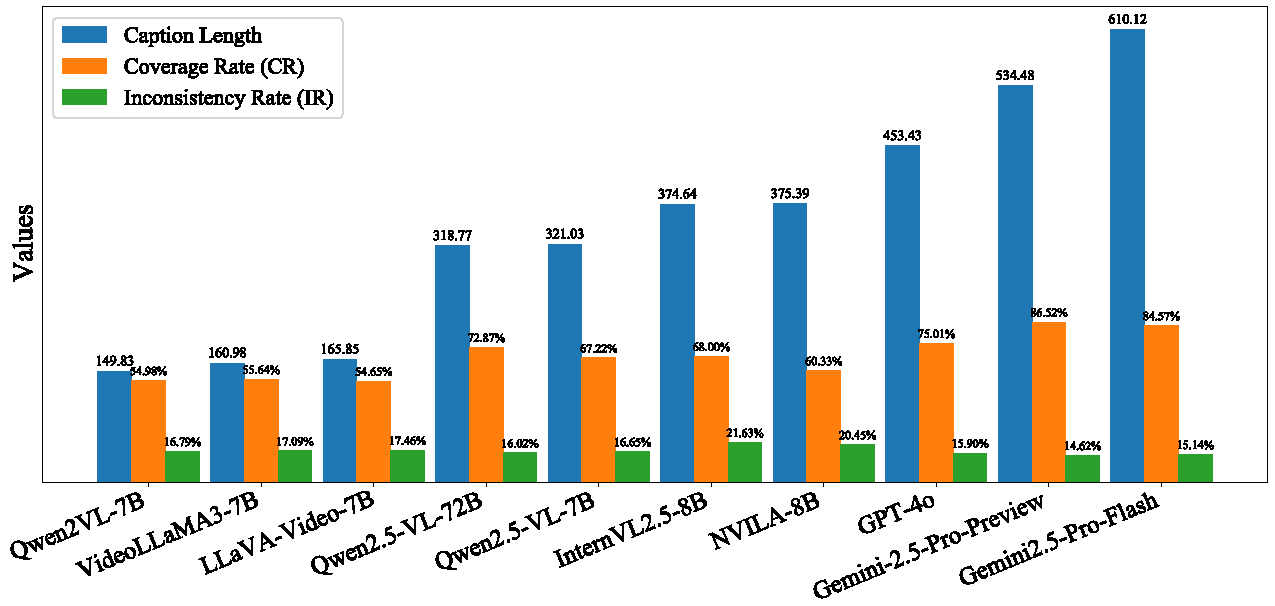
\includegraphics[width=1.0\linewidth]{imgs/comparison_chart_sorted_NEW11.pdf}
    \vspace{-0.5em}
	\caption{The relationship between CR, IR and caption length, where Gemini-2.5-Pro-Preview as a TextQA expert. Caption length is the number of words in the caption, not counting special symbols.}
	\label{fig:fig7}
	\end{minipage}%
	\vspace{-1.5em}	
\end{figure}


\subsection{Main Results}

\textbf{Accuracy (AR):} As illustrated in Table~\ref{tab:results_1} and Fig.~\ref{fig:fig6}, Gemini-2.5-Pro-Preview consistently surpasses all other models across various dimensions when evaluated using the Accuracy (AR) metric. For instance, in the ``Content \& Entity" dimension, specifically concerning action, Gemini-2.5-Pro-Preview achieves an AR of 74.13\%, whereas other models typically fall between 40\% and 70\%. In the ``Color \& Light" dimension, particularly for lighting, Gemini-2.5-Pro-Preview records an impressive AR of 79.67\%, significantly outperforming its counterparts. When considering the entire dataset, Gemini-2.5-Pro-Preview achieves an AR of 73.88\%, which is markedly superior to that of other open-source models. Among these, the latest Qwen2.5-VL-72B shows the best performance with an AR of 61.20\%, yet it remains considerably lower than Gemini-2.5-Pro-Preview. This underscores Gemini-2.5-Pro-Preview's exceptional ability to accurately capture and describe video content, thereby delivering higher quality descriptions and insights.


\textbf{Inconsistency Rate (IR):} Gemini-2.5-Pro-Preview stands out in terms of the IR metric, achieving the lowest IR values. For instance, in the ``Visuals \& Composition'' category, especially for background, Gemini-2.5-Pro-Preview records an IR of just 9.76\%, while other models typically range between 10\% and 20\%. In the ``Cinematography \& Environment'' category, especially for lighting, Gemini-2.5-Pro-Flash's IR is only 14.22\%.

\textbf{Coverage Rate (CR):} When it comes to the CR metric, Gemini-2.5-Pro-Preview again shows superior performance. In the ``Content \& Entity'' category, the lowest CR for Gemini-2.5-Pro-Preview is 61.12\% in the ``Entity Shape'' subcategory, while the highest is 90.12\% in the ``Entity'' subcategory. Other open-source models have CR values that are more than 10\% lower across all categories. Overall, Gemini-2.5-Pro-Preview achieves an impressive CR of 86.52\%. Among open-source models, InternVL2.5-8B performs best with a CR of 68.00\%, which is 18.52\% lower than Gemini-2.5-Pro-Preview. This demonstrates that Gemini-2.5-Pro-Preview can cover more relevant content from the video, providing more comprehensive coverage regardless of description consistency. 

Gemini-2.5-Pro-Preview excels in generating video descriptions, demonstrating high accuracy (AR), consistency (IR), and comprehensive coverage (CR). This underscores its superior performance in producing high-quality, detailed, and consistent descriptions compared to other models. VCapsBench highlights the shortcomings of existing open-source VLMs, such as the lack of detailed object shapes, sizes, colors, and lighting in descriptions. These deficiencies can be particularly problematic for applications requiring highly detailed and complete captions, such as text-to-video generation models and advanced video analysis tools.


\subsection{Evaluation Analysis}
Although Gemini surpasses open-source VLMs in every aspect, showcasing its advanced video comprehension abilities, it is crucial to acknowledge that Gemini's captions were utilized in creating QA-pairs, potentially influencing its elevated CR. Nevertheless, Gemini's metrics are valuable as they establish a benchmark for open-source models, emphasizing the disparity in video content understanding. This insight is instrumental in guiding the optimization of open-source VLMs.

\begin{figure*}[thbp]
	\begin{minipage}[t]{1.0\linewidth}%\centering
	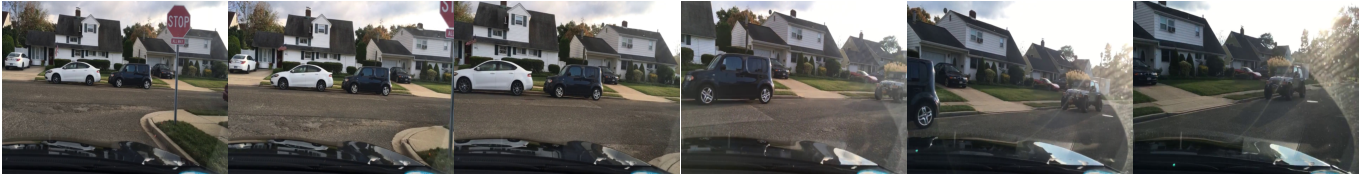
\includegraphics[width=1\linewidth]{imgs/exp_video3.pdf}
    \vspace{-1.5em}
     \caption{Representative video from VCapsBench.}
	\label{fig:fig9}
	\end{minipage}%
	\vspace{-1.5em}	
\end{figure*}

\begin{table*}[htbp]
\centering
\setlength{\tabcolsep}{6pt}
\renewcommand{\arraystretch}{0.8}
\caption{Questions for representative video from VCapsBench. ``Q2.5-72B", ``LV-7B", ``Q2-7B", ``VL-7B", ``NV-8B", ``I2.5-8B", ``Q2.5-7B", ``G2.5" represent ``Qwen2.5VL-72B", ``LLaVA-Video-7B", ``Qwen2VL-7B", ``VideoLLaMA3-7B", ``NVILA-8B", ``InternVL2.5-8B", ``Qwen2.5VL-7B" and ``Gemini-2.5-Pro-Preview" respectively. ``\CheckmarkBold", ``\XSolidBrush", ``\boldmath $\bullet$" represent ``Positive", ``Negative" and ``Unanswerable", respectively.}
\resizebox{\textwidth}{!}{%
\begin{tabular}{l|l|p{9.2cm}|c|cccccccc}
\toprule 
    % &Category & Question & GT & \begin{tabular}[c]{@{}c@{}}\small Qwen2VL\\ \small 72B\end{tabular} & 
    % \begin{tabular}[c]{@{}c@{}}\small LLaVA\\ \small Video-7B\end{tabular} & \begin{tabular}[c]{@{}c@{}}\small Qwen2VL\\ \small 7B\end{tabular} & \begin{tabular}[c]{@{}c@{}}\small VideoLLaMA3\\ \small 7B\end{tabular}
    % & \begin{tabular}[c]{@{}c@{}}\small NVILA\\ \small 8B\end{tabular} & \begin{tabular}[c]{@{}c@{}}\small InternVL2.5\\ \small 8B\end{tabular}& \begin{tabular}[c]{@{}c@{}}\small Qwen2.5VL\\ \small 7B\end{tabular} & \small Gemini-1.5\\ 
    &Category & Question & GT & \small Q2.5-72B &\small LV-7B& \small Q2-7B & \small VL-7B
    & \small NV-8B & \small I2.5-8B & \small Q2.5-7B & \small G2.5\\ 
    \midrule
    \multirow{7}{*}{\rotatebox{90}{\begin{tabular}[c]{@{}c@{}}\small Content\\ \small  \& Entity \end{tabular} }}
    &action & Is there a subtle panning movement from left to right in the video? & yes & \CheckmarkBold & \XSolidBrush & \XSolidBrush & \CheckmarkBold & \boldmath $\bullet$ & \CheckmarkBold & \CheckmarkBold & \CheckmarkBold\\
    \cline{2-4} 
    &count & Are there more than three cars visible in the video? & yes & \boldmath $\bullet$ &  \CheckmarkBold &  \CheckmarkBold & \CheckmarkBold & \CheckmarkBold & \CheckmarkBold & \CheckmarkBold & \CheckmarkBold\\
    \cline{2-4} 
    &relation & Is the red car parked on the opposite side of the street? & yes & \boldmath $\bullet$ &  \boldmath $\bullet$& \CheckmarkBold  & \boldmath $\bullet$ & \boldmath $\bullet$ &\XSolidBrush &\boldmath $\bullet$ &\XSolidBrush\\
    \cline{2-4} 
    &entity& Is there a stop sign in the video? & yes &  \CheckmarkBold & \CheckmarkBold & \CheckmarkBold & \CheckmarkBold &\CheckmarkBold &\CheckmarkBold &\CheckmarkBold &\CheckmarkBold\\
    \cline{2-4} 
    &entity size & Is the black SUV larger than the white sedan? & yes & \boldmath $\bullet$ &  \boldmath $\bullet$ & \boldmath $\bullet$ &\boldmath $\bullet$  &\boldmath $\bullet$ &\boldmath $\bullet$ &\boldmath $\bullet$ &\boldmath $\bullet$\\
    \cline{2-4} 
    &entity shape& Is the stop sign octagonal? & yes & \boldmath $\bullet$ & \boldmath $\bullet$ & \CheckmarkBold & \boldmath $\bullet$ &\boldmath $\bullet$ & \boldmath $\bullet$ &\boldmath $\bullet$ & \CheckmarkBold\\
     \midrule
    \multirow{6}{*}{\rotatebox{90}{\begin{tabular}[c]{@{}c@{}}\small Color\\ \small  \& Light \end{tabular}}}
    &lighting & \begin{tabular}[l]{@{}l@{}}Is the lighting in video primarily natural and even, \\ characteristic of daytime? \end{tabular}& yes &  \CheckmarkBold & \boldmath $\bullet$ & \XSolidBrush & \boldmath $\bullet$ & \CheckmarkBold & \CheckmarkBold & \CheckmarkBold &  \CheckmarkBold \\
    \cline{2-4} 
    &color palette & Does the video have a realistic color palette? & yes & \CheckmarkBold &  \CheckmarkBold &\boldmath $\bullet$ & \boldmath $\bullet$ & \boldmath $\bullet$ &\CheckmarkBold &\CheckmarkBold &  \CheckmarkBold\\
    \cline{2-4} 
    &color grading & Is the image ungraded, with natural tones for the houses and cars? & yes & \boldmath $\bullet$ &  \CheckmarkBold &\boldmath $\bullet$ & \boldmath $\bullet$ & \boldmath $\bullet$ &\CheckmarkBold & \boldmath $\bullet$  &  \CheckmarkBold \\
    \cline{2-4} 
    &color &Is the white sedan parked directly in front of the stop sign? & yes & \boldmath $\bullet$ &  \boldmath $\bullet$ &  \CheckmarkBold &  \boldmath $\bullet$ & \XSolidBrush & \XSolidBrush & \boldmath $\bullet$ & \boldmath $\bullet$\\
    \midrule
    \multirow{6}{*}{\rotatebox{90}{\begin{tabular}[c]{@{}c@{}}\small Visuals \& \\ \small Composition \end{tabular}}}&position & Is the stop sign on the right side of the road? & yes & \boldmath $\bullet$ & \CheckmarkBold & \CheckmarkBold & \boldmath $\bullet$ & \CheckmarkBold & \CheckmarkBold &\boldmath $\bullet$ & \boldmath $\bullet$\\
    \cline{2-4} 
    &relative position & Is the white car closer to the stop sign than the black car? & no & \boldmath $\bullet$ &  \boldmath $\bullet$ & \XSolidBrush & \boldmath $\bullet$ &\boldmath $\bullet$ &\boldmath $\bullet$ & \boldmath $\bullet$ &\boldmath $\bullet$\\
    \cline{2-4} 
    &background & Is the video set in a residential suburban street? & yes & \CheckmarkBold & \CheckmarkBold & \CheckmarkBold & \CheckmarkBold & \CheckmarkBold & \CheckmarkBold & \CheckmarkBold &  \CheckmarkBold \\
    \cline{2-4} 
    &text & Is there a stop sign with the text ``ALL WAY" in the video? & yes & \CheckmarkBold & \XSolidBrush & \CheckmarkBold   & \CheckmarkBold & \CheckmarkBold & \XSolidBrush & \CheckmarkBold & \boldmath $\bullet$\\
    \cline{2-4} 
    &blur & Is there a shallow depth of field in the video? & yes & \boldmath $\bullet$ &  \CheckmarkBold &\boldmath $\bullet$ & \boldmath $\bullet$ & \boldmath $\bullet$ & \boldmath $\bullet$ & \boldmath $\bullet$ &  \CheckmarkBold \\
    \midrule
    \multirow{3}{*}{\rotatebox{90}{ \begin{tabular}[c]{@{}c@{}}\small Cinematography\\ \small  \& Environment \end{tabular}}}&camera movement & Is the camera movement in the video a slow panning from left to right? & yes & \CheckmarkBold & \XSolidBrush & \XSolidBrush & \CheckmarkBold & \boldmath $\bullet$ & \boldmath $\bullet$ & \XSolidBrush &  \CheckmarkBold\\
    \cline{2-4} 
    &shot type& Is the primary shot type predominantly a medium shot taken from a fixed perspective? & yes & \boldmath $\bullet$ & \XSolidBrush & \XSolidBrush & \boldmath $\bullet$ & \boldmath $\bullet$ & \XSolidBrush & \XSolidBrush &  \CheckmarkBold \\
    \cline{2-4} 
    &atmosphere & Is the video set in a calm and quiet atmosphere, typical of a residential neighborhood?  & yes & \CheckmarkBold & \CheckmarkBold  & \CheckmarkBold & \CheckmarkBold & \XSolidBrush & \XSolidBrush & \CheckmarkBold & \CheckmarkBold \\
\bottomrule
\end{tabular}
}
\label{tbl:bench_questions}
\vspace{-1.0em}	
\end{table*}



\textbf{Caption length distribution analysis.} We also explore the caption lengths to determine if longer captions are associated with a higher evaluation coverage rate (CR), as shown in Fig.~\ref{fig:fig7} . The Fig.~\ref{fig:fig11} in Appendix \ref{exp_app} presents histograms of caption word lengths for the models assessed. Our findings indicate that as the length of captions generated by models increases, the CR generally improves. However, this increase in length also leads to more errors in some open-source models, such as Qwen2VL-7B, VideoLLaMA3-7B, LLaVA-Video-7B, and InternVL2.5-8B. Interestingly, open-source VLMs like Qwen2.5-VL-72B and the closed VLM Gemini-2.5, despite producing longer captions, exhibit lower error rates compared to other VLMs. Additionally, Qwen2.5-VL-7B achieves a higher CR than VILA-8B with shorter captions and a lower IR than LLaVA-Video-7B, which also has shorter captions. This suggests that a deep understanding of video content allows models to generate concise, yet thorough and accurate descriptions.


\textbf{Representative sample analysis.} To further examine the strengths and weaknesses of various models, we conducted a qualitative analysis of captions. In Fig.~\ref{fig:fig9}, we present a video from VCapsBench, which features numerous subjects and intricate details, posing a significant challenge for VLMs. Table.~\ref{tbl:bench_questions} lists the questions for this video along with the answers derived from the captions. It is evident that different VLMs exhibit varying performances across different dimensions. Some categories, such as ``atmosphere'' and ``background'' are relatively easy for all VLMs, whereas others, like ``relative position'' present difficulties for all models. However, each video has unique questions across different categories. The comprehensive dataset includes a vast number of questions, sufficient to thoroughly evaluate a VLM's capability to understand and observe video details. More results in Appendix \ref{exp_app}, \ref{exp_app1} and \ref{exp_app2}.




\section{Conclusion}
In this work, we introduce VCapsBench, a new large-scale fine-grained benchmark for evaluating video caption quality. VCapsBench is meticulously designed to support detailed long captions, aiming to advance research and benchmarking in video understanding. The benchmark comprises over 5K videos and more than 100K QA-pairs, assessing 21 critical dimensions of video generation. We have evaluated the caption quality produced by various open-source and closed-source models using this benchmark. The comprehensive analysis highlights the strengths and weaknesses of these models in generating accurate and detailed captions. We believe that VCapsBench will play a crucial role in guiding the optimization of video caption generation, thereby advancing the development of text-to-video models and enhancing the overall understanding of video content.





\clearpage
\bibliography{
neurips_2025
}

\clearpage
\appendix
\section{Technical Appendices and Supplementary Material}
In this section, we present the automated evaluation results, employing GPT-4.1 as the evaluation expert. This analysis aims to provide researchers with deeper insights into the characteristics of our dataset, as well as the variations in outcomes attributable to different evaluation experts. Additionally, we include the original caption outputs and corresponding evaluation results produced by various models for comprehensive comparison.


\subsection{More Experimental Results With GPT-4.1}\label{exp_app}

\begin{table*}[htbp]
\renewcommand{\arraystretch}{0.6}
\caption{The accuracy (AR), inconsistency rate (IR), and coverage rate (CR) of VLM methods on all dimensions, where GPT-4.1 as a TextQA expert. The symbol ``$\uparrow$"  indicates that the larger the value, the better; The symbol ``$\downarrow$" indicates that the smaller the value, the better.}
\label{tab:results_2}
\resizebox{\textwidth}{!}{%
\begin{tabular}{@{}ll|cccccccccccc@{}}
\toprule
 &\multirow{3}{*}{Methods}& \multicolumn{7}{c|}{Content \& Entity}& \multicolumn{4}{c}{Color \&  Light}\\
 \cline{3-13} 
 &  & \begin{tabular}[c]{@{}c@{}}\small Proper\\ \small Noun\end{tabular} & \begin{tabular}[c]{@{}c@{}}Action\end{tabular} & \begin{tabular}[c]{@{}c@{}}Relation
\end{tabular} & \begin{tabular}[c]{@{}c@{}}Count
\end{tabular} & Entity  & \begin{tabular}[c]{@{}c@{}}\small Entity\\ \small Size\end{tabular} & \multicolumn{1}{c|}{\begin{tabular}[c]{@{}c@{}}\small Entity\\ \small Shape\end{tabular} }
&\begin{tabular}[c]{@{}c@{}}Lighting
\end{tabular} & \begin{tabular}[c]{@{}c@{}}\small Color \\ \small Palette \end{tabular} & \begin{tabular}[c]{@{}c@{}}\small Color\\ \small Grading
\end{tabular} & \begin{tabular}[c]{@{}c@{}}Color
\end{tabular}  \\ \midrule
\multirow{8}{*}{\rotatebox{90}{AR}$\Bigg\uparrow$} 
& LLaVA-Video-7B & 40.73 & 57.08 & 51.67 & 54.88 & 34.02 & 66.2 & \multicolumn{1}{c|}{26.62} & 57.59 & 61.49 & 23.78 & 55.97 \\
& Qwen2VL-7B & 39.17 & 56.32 & 52.87 & 57.17 & 32.27 & 64.2 & \multicolumn{1}{c|}{25.61} & 69.93 & 55.57 & 30.62 & \multicolumn{1}{c|}{50.75}  \\ 
& VideoLLaMA3-7B & 38.92 & 58.51 & 52.56 & 56.27 & 33.48 & 64.28 & \multicolumn{1}{c|}{25.56} & 60.59 & 59.03 & 25.24 & \multicolumn{1}{c|}{54.12}\\
& NVILA-8B & 40.03 & 44.2 & 48.04 & 57.9 & 37.3 & 63.72 & \multicolumn{1}{c|}{29.32} & 72.63 & 66.01 & 42.37 & \multicolumn{1}{c|}{59.35} \\ 
& InternVL2.5-8B & 38.63 & 53.86 & 48.71 & 59.64 & 36.78 & 60.91 & \multicolumn{1}{c|}{29.44} & 81.27 & 75.35 & 60.36 & \multicolumn{1}{c|}{55.82} \\
& Qwen2.5VL-7B & 46.95 & 63.86 & 57.72 & 62.39 & 41.75 & 69.35 & \multicolumn{1}{c|}{34.89} & 83.6 & 73.9 & 51.32 & \multicolumn{1}{c|}{59.8}  \\ 
& Qwen2.5-VL-72B & 48.76 & 67.28 & 63.03 & 67.33 & 45.37 & 72.51 & \multicolumn{1}{c|}{37.76} & 88.42 & 75.28 & 61.31 & \multicolumn{1}{c|}{62.69}  \\ 
& GPT-4o  & 51.11 & 69.48 & 66.34 & 70.08 & 51.38 & 77.5 & \multicolumn{1}{c|}{47.89} & 87.96 & 82.47 & 68.17 & \multicolumn{1}{c|}{67.07} \\ 
& Gemini2.5-Pro-Flash & 60.21 & 76.23 & 73.54 & 79.59 & 63.97 & 85.25 & \multicolumn{1}{c|}{59.55} & \textbf{90.05} & 86.57 & \textbf{69.06} & \multicolumn{1}{c|}{79.36}\\ 
& Gemini-2.5-Pro-Preview & \textbf{61.41} & \textbf{78.13} & \textbf{75.19} & \textbf{80.54} & \textbf{64.4} & \textbf{86.52} & \multicolumn{1}{c|}{\textbf{62.21}} & 88.9 & \textbf{88.06} & 66.95 & \multicolumn{1}{c|}{\textbf{79.96}} \\ 

\midrule
\multirow{8}{*}{\rotatebox{90}{IR}$\Bigg\downarrow$} 
& LLaVA-Video-7B & 13.09 & 15.13 & 11.29 & 13.14 & 3.76 & 8.62 & \multicolumn{1}{c|}{8.45} & \textbf{5.62} & 11.05 & \textbf{4.12} & \multicolumn{1}{c|}{13.23} \\
& Qwen2VL-7B & 8.38 & 13.84 & 10.27 & 11.67 & 3.77 & 8.64 & \multicolumn{1}{c|}{\textbf{6.05}} & 7.26 & 12.88 & 5.67 & \multicolumn{1}{c|}{13.44} \\
& VideoLLaMA3-7B & 9.91 & 17.88 & 11.99 & 12.59 & 3.46 & 8.41 & \multicolumn{1}{c|}{7.56} & 6.19 & 11.49 & 4.39 & \multicolumn{1}{c|}{12.77}  \\
& NVILA-8B & 11.88 & 20.21 & 14.96 & 15.45 & 4.48 & 12.42 & \multicolumn{1}{c|}{9.61} & 8.08 & 15.72 & 6.52 & \multicolumn{1}{c|}{17.75}  \\
& InternVL2.5-8B & 14.57 & 19.0 & 16.43 & 14.18 & 5.5 & 14.0 & \multicolumn{1}{c|}{10.23} & 8.06 & 15.11 & 8.57 & \multicolumn{1}{c|}{16.01} \\
& Qwen2.5VL-7B & 8.65 & 14.66 & 12.39 & 11.35 & \textbf{3.16} & 9.25 & \multicolumn{1}{c|}{8.38} & 6.9 & 11.5 & 5.52 & \multicolumn{1}{c|}{13.87} \\

& Qwen2.5-VL-72B & 7.86 & 15.0 & 11.58 & 11.66 & 5.02 & 8.96 & \multicolumn{1}{c|}{8.28} & 6.89 & 13.44 & 5.3 & \multicolumn{1}{c|}{15.23} \\ 
& GPT-4o & 7.53 & \textbf{11.26} & \textbf{9.56} & 10.45 & 3.94 & 6.5 & \multicolumn{1}{c|}{8.48} & 6.34 & 11.69 & 7.32 & \multicolumn{1}{c|}{13.15} \\ 
& Gemini2.5-Pro-Flash & 6.76 & 12.59 & 9.57 & 9.81 & 5.23 & \textbf{5.36} & \multicolumn{1}{c|}{8.43} & 6.43 & 11.32 & 6.98 & \multicolumn{1}{c|}{\textbf{11.19}} \\
& Gemini-2.5-Pro-Preview & \textbf{6.58}& 13.06 & 9.77 & \textbf{9.06} & 4.29 & 5.88 & \multicolumn{1}{c|}{8.64} & 7.08 & \textbf{10.16} & 5.76 & \multicolumn{1}{c|}{12.18}\\ 

 \midrule
\multirow{8}{*}{\rotatebox{90}{CR}$\Bigg\uparrow$} 
& LLaVA-Video-7B & 46.87 & 67.25 & 58.25 & 63.17 & 35.35 & 72.44 & \multicolumn{1}{c|}{29.07} & 61.03 & 69.13 & 24.81 & \multicolumn{1}{c|}{64.51}   \\
& Qwen2VL-7B & 42.75 & 65.36 & 58.92 & 64.73 & 33.54 & 70.27 & \multicolumn{1}{c|}{27.26} & 75.41 & 63.79 & 32.46 & \multicolumn{1}{c|}{58.63}  \\ 
& VideoLLaMA3-7B & 43.2 & 71.25 & 59.72 & 64.38 & 34.68 & 70.19 & \multicolumn{1}{c|}{27.65} & 64.59 & 66.7 & 26.4 & \multicolumn{1}{c|}{62.05}  \\
& NVILA-8B & 45.43 & 55.4 & 56.49 & 68.48 & 39.05 & 72.76 & \multicolumn{1}{c|}{32.43} & 79.01 & 78.33 & 45.32 & \multicolumn{1}{c|}{72.16}  \\
& InternVL2.5-8B & 45.22 & 66.49 & 58.29 & 69.49 & 38.92 & 70.82 & \multicolumn{1}{c|}{32.8} & 88.4 & 88.75 & 66.02 & \multicolumn{1}{c|}{66.46}   \\
& Qwen2.5VL-7B & 51.4 & 74.83 & 65.88 & 70.37 & 43.11 & 76.42 & \multicolumn{1}{c|}{38.08} & 89.79 & 83.5 & 54.32 & \multicolumn{1}{c|}{69.43} \\ 
& Qwen2.5-VL-72B & 52.92 & 79.16 & 71.28 & 76.21 & 47.76 & 79.64 & \multicolumn{1}{c|}{41.17} & 94.96 & 86.97 & 64.74 & \multicolumn{1}{c|}{73.96}  \\ 

& GPT-4o & 55.27 & 78.3 & 73.36 & 78.26 & 53.48 & 82.89 & \multicolumn{1}{c|}{52.33} & 93.92 & 93.39 & 73.56 & \multicolumn{1}{c|}{77.23}\\ 
& Gemini2.5-Pro-Flash & 64.58 & 87.22 & 81.32 & 88.25 & \textbf{67.5} & 90.07 & \multicolumn{1}{c|}{65.03} & \textbf{96.24} & 97.62 & \textbf{74.24} & \multicolumn{1}{c|}{89.36}\\ 
& Gemini-2.5-Pro-Preview & \textbf{65.73} & \textbf{89.86} & \textbf{83.33} & \textbf{88.56} & 67.28 & \textbf{91.93} & \multicolumn{1}{c|}{\textbf{68.1}} & 95.68 & \textbf{98.02} & 71.04 & \multicolumn{1}{c|}{\textbf{91.04}} \\ 


 \bottomrule
 \toprule
 &\multirow{3}{*}{Methods}& \multicolumn{5}{c|}{Visuals \& Composition}& \multicolumn{5}{c|}{Cinematography  \& Environment}\\
 \cline{3-13} 
 &  & Position & \begin{tabular}[c]{@{}c@{}}\small Relative\\ \small Position\end{tabular} & Background &Text & \multicolumn{1}{c|}{Blur} & Style & \begin{tabular}[c]{@{}c@{}}\small Camera \\ \small Movement\end{tabular} & \begin{tabular}[c]{@{}c@{}}Shot Type\end{tabular} & \begin{tabular}[c]{@{}c@{}}Emotion\end{tabular} & \multicolumn{1}{c|}{Atmosphere} & \color{red}\textbf{ALL}\\ \midrule
\multirow{8}{*}{\rotatebox{90}{AR}$\Bigg\uparrow$} 

& LLaVA-Video-7B & 34.26 & 32.96 & 69.28 & 43.75 & \multicolumn{1}{c|}{13.49} & 66.6 & 23.68 & 38.13 & 48.53 & \multicolumn{1}{c|}{82.04} & 47.74 \\
& Qwen2VL-7B & 35.34 & 32.4 & 68.69 & 34.75 & \multicolumn{1}{c|}{15.17} & 71.53 & 16.26 & 32.7 & 55.24 & \multicolumn{1}{c|}{83.56} & 47.45\\ 
& VideoLLaMA3-7B & 35.41 & 32.54 & 65.35 & 38.11 & \multicolumn{1}{c|}{16.99} & 71.66 & 39.32 & 39.53 & 53.27 & \multicolumn{1}{c|}{80.44} &48.45  \\
& NVILA-8B & 40.69 & 33.36 & 69.7 & 38.04 & \multicolumn{1}{c|}{26.42} & 74.11 & 16.97 & 39.4 & 53.46 & \multicolumn{1}{c|}{81.02} &49.70 \\
& InternVL2.5-8B & 39.08 & 32.59 & 70.89 & 37.31 & \multicolumn{1}{c|}{36.83} & 86.59 & 51.3 & 50.53 & 58.75 & \multicolumn{1}{c|}{86.57} &54.85  \\
 & Qwen2.5VL-7B & 45.0 & 38.58 & 77.18 & 44.96 & \multicolumn{1}{c|}{30.71} & 88.55 & 51.92 & 50.9 & 63.5 & \multicolumn{1}{c|}{89.51} &58.74 \\ 
& Qwen2.5-VL-72B & 49.83 & 43.01 & 78.99 & 45.55 & \multicolumn{1}{c|}{36.31} & 92.0 & 66.47 & 59.37 & 67.78 & \multicolumn{1}{c|}{89.91} &63.08 \\
& GPT-4o & 57.24 & 49.0 & 83.14 & 46.79 & \multicolumn{1}{c|}{48.0} & 92.05 & 55.57 & 62.97 & 62.45 & \multicolumn{1}{c|}{\textbf{90.82}} &66.49\\
& Gemini2.5-Pro-Flash & 70.36 & 63.56 & 87.64 & \textbf{63.7} & \multicolumn{1}{c|}{67.33} & \textbf{96.13} & 70.76 & 74.29 & 73.01 & \multicolumn{1}{c|}{86.22} &75.56 \\
& Gemini-2.5-Pro-Preview & \textbf{70.63} & \textbf{66.11} & \textbf{87.97} & 63.5 & \multicolumn{1}{c|}{\textbf{68.75}} & 95.76 & \textbf{74.89} & \textbf{75.72} & \textbf{77.05} & \multicolumn{1}{c|}{88.34} &\color{red}\textbf{76.73}\\


 \midrule
\multirow{8}{*}{\rotatebox{90}{IR}$\Bigg\downarrow$} 
& LLaVA-Video-7B & \textbf{10.46} & 11.83 & 7.5 & 17.92 & \multicolumn{1}{c|}{\textbf{10.11}} & \textbf{1.64} & 24.13 & \textbf{12.18} & \textbf{3.67} & \multicolumn{1}{c|}{\textbf{3.71}} & 10.05\\
& Qwen2VL-7B & 11.18 & \textbf{10.39} & 8.8 & 13.47 & \multicolumn{1}{c|}{14.47} & 2.72 & 19.21 & 13.17 & 5.16 & \multicolumn{1}{c|}{6.25} & \color{red}\textbf{9.65} \\
& VideoLLaMA3-7B & 12.26 & 12.21 & 7.94 & 14.86 & \multicolumn{1}{c|}{12.18} & 2.22 & 23.44 & 14.68 & 3.74 & \multicolumn{1}{c|}{4.52} &10.50\\
& NVILA-8B & 16.22 & 16.46 & 10.26 & 17.93 & \multicolumn{1}{c|}{18.62} & 4.51 & 23.6 & 22.5 & 6.31 & \multicolumn{1}{c|}{6.05} &13.12\\
& InternVL2.5-8B & 15.32 & 14.72 & 8.74 & 19.13 & \multicolumn{1}{c|}{21.88} & 4.89 & 26.24 & 20.04 & 6.11 & \multicolumn{1}{c|}{5.57} &13.41 \\
& Qwen2.5VL-7B & 12.8 & 13.45 & 8.37 & 12.25 & \multicolumn{1}{c|}{19.8} & 2.72 & 22.77 & 16.43 & 5.47 & \multicolumn{1}{c|}{5.09} & 10.62\\

& Qwen2.5-VL-72B & 13.34 & 13.5 & 7.98 & 12.56 & \multicolumn{1}{c|}{20.73} & 3.36 & 20.99 & 16.97 & 5.56 & \multicolumn{1}{c|}{5.14} &10.98\\
& GPT-4o & 12.42 & 12.35 & 6.23 & 12.9 & \multicolumn{1}{c|}{22.32} & 3.64 & 21.35 & 19.02 & 6.91 & \multicolumn{1}{c|}{5.06} &10.24\\

&  Gemini2.5-Pro-Flash & 14.68 & 15.16 & \textbf{5.05} & 11.87 & \multicolumn{1}{c|}{23.45} & 2.25 & 20.57 & 20.34 & 5.12 & \multicolumn{1}{c|}{4.79} &10.49\\

&Gemini-2.5-Pro-Preview & 15.65 & 13.98 & 5.12 & \textbf{10.92} & \multicolumn{1}{c|}{22.58} & 2.33 & \textbf{18.68} & 19.17 & 4.7 & \multicolumn{1}{c|}{4.7} &10.28\\

 \midrule
\multirow{8}{*}{\rotatebox{90}{CR}$\Bigg\uparrow$} 
& LLaVA-Video-7B & 38.26 & 37.38 & 74.9 & 53.3 & \multicolumn{1}{c|}{15.01} & 67.71 & 31.22 & 43.42 & 50.38 & \multicolumn{1}{c|}{85.2} & 53.08\\
& Qwen2VL-7B & 39.79 & 36.16 & 75.32 & 40.16 & \multicolumn{1}{c|}{17.74} & 73.53 & 20.13 & 37.66 & 58.25 & \multicolumn{1}{c|}{89.14}  & 52.52\\ 
& VideoLLaMA3-7B & 40.36 & 37.07 & 70.98 & 44.76 & \multicolumn{1}{c|}{19.35} & 73.29 & 51.37 & 46.33 & 55.34 & \multicolumn{1}{c|}{84.25}  & 54.13\\
& NVILA-8B & 48.57 & 39.93 & 77.67 & 46.35 & \multicolumn{1}{c|}{32.46} & 77.61 & 22.22 & 50.83 & 57.06 & \multicolumn{1}{c|}{86.24}  & 57.21\\
& InternVL2.5-8B & 46.15 & 38.22 & 77.69 & 46.14 & \multicolumn{1}{c|}{47.14} & 91.05 & 69.55 & 63.19 & 62.57 & \multicolumn{1}{c|}{91.68} & 63.34\\
& Qwen2.5VL-7B & 51.6 & 44.58 & 84.23 & 51.24 & \multicolumn{1}{c|}{38.3} & 91.03 & 67.23 & 60.91 & 67.17 & \multicolumn{1}{c|}{94.31} &65.75 \\
& Qwen2.5-VL-72B & 57.5 & 49.72 & 85.84 & 52.1 & \multicolumn{1}{c|}{45.81} & 95.2 & 84.14 & 71.51 & 71.78 & \multicolumn{1}{c|}{94.78} &70.86\\
& GPT-4o & 65.36 & 55.91 & 88.67 & 53.72 & \multicolumn{1}{c|}{61.8} & 95.52 & 70.65 & 77.77 & 67.09 & \multicolumn{1}{c|}{\textbf{95.66}} &74.07\\
& Gemini2.5-Pro-Flash & 82.47 & 74.92 & 92.3 & \textbf{72.27} & \multicolumn{1}{c|}{87.96} & \textbf{98.35} & 89.09 & 93.26 & 76.95 & \multicolumn{1}{c|}{90.55} &84.42\\
& Gemini-2.5-Pro-Preview & \textbf{83.74} & \textbf{76.86} & \textbf{92.72} & 71.28 & \multicolumn{1}{c|}{\textbf{88.8}} & 98.04 & \textbf{92.09} & \textbf{93.68} & \textbf{80.85} & \multicolumn{1}{c|}{92.7}&\color{red}\textbf{85.52} \\

\bottomrule
\end{tabular}%
}
\end{table*}

\begin{figure*}[tp]
	\begin{minipage}[t]{1.0\linewidth}
        \centering
	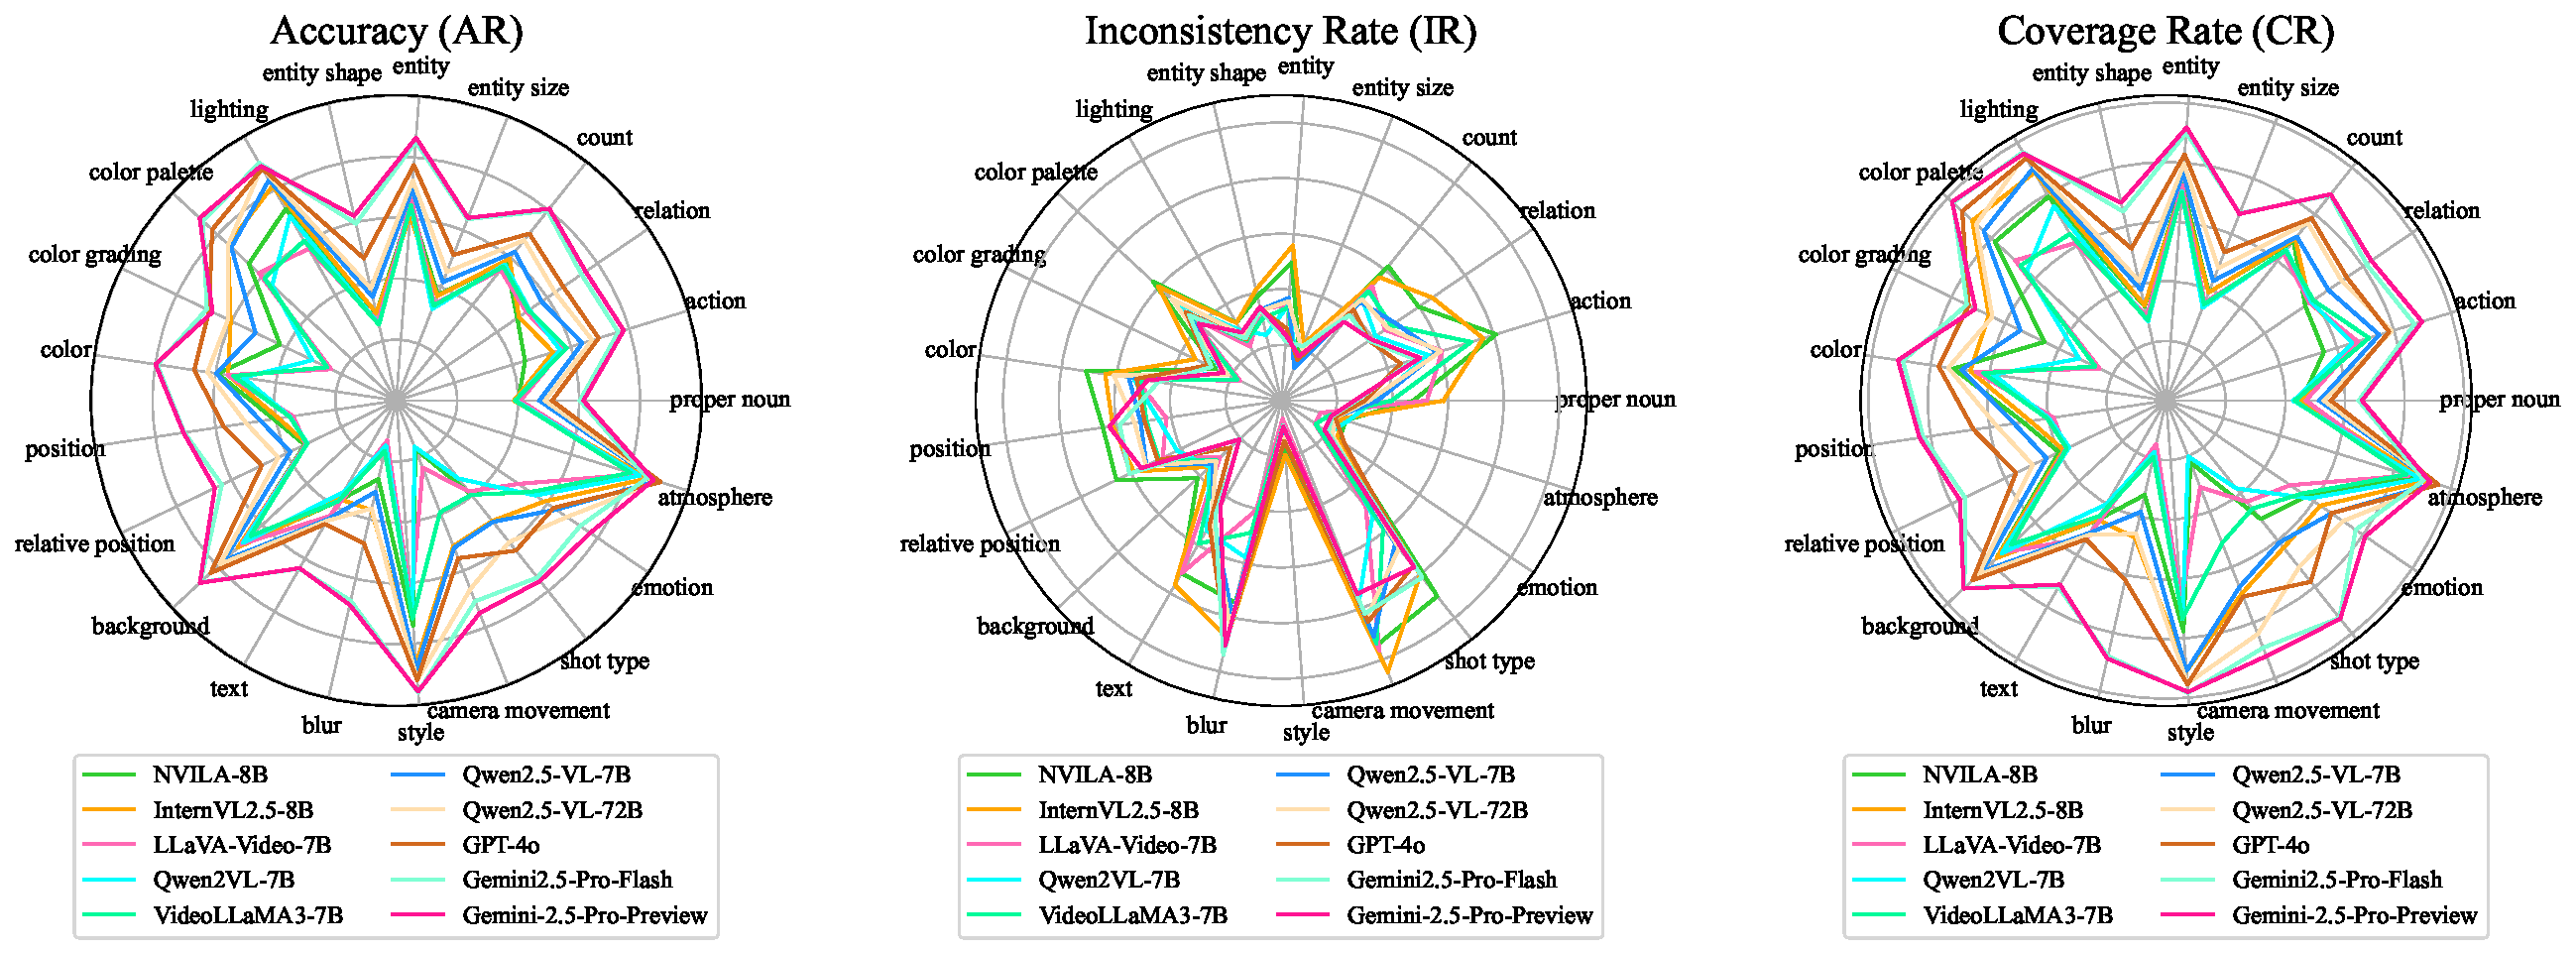
\includegraphics[width=1.0\linewidth]{imgs/radar_chart_all-New2.pdf}
	\caption{Results of GPT-4.1 captioning evaluation, organized by category.}
	\label{fig:fig9}
	\end{minipage}%
\end{figure*}

\begin{figure}[thbp]
	\begin{minipage}[t]{1.0\linewidth}
        \centering
	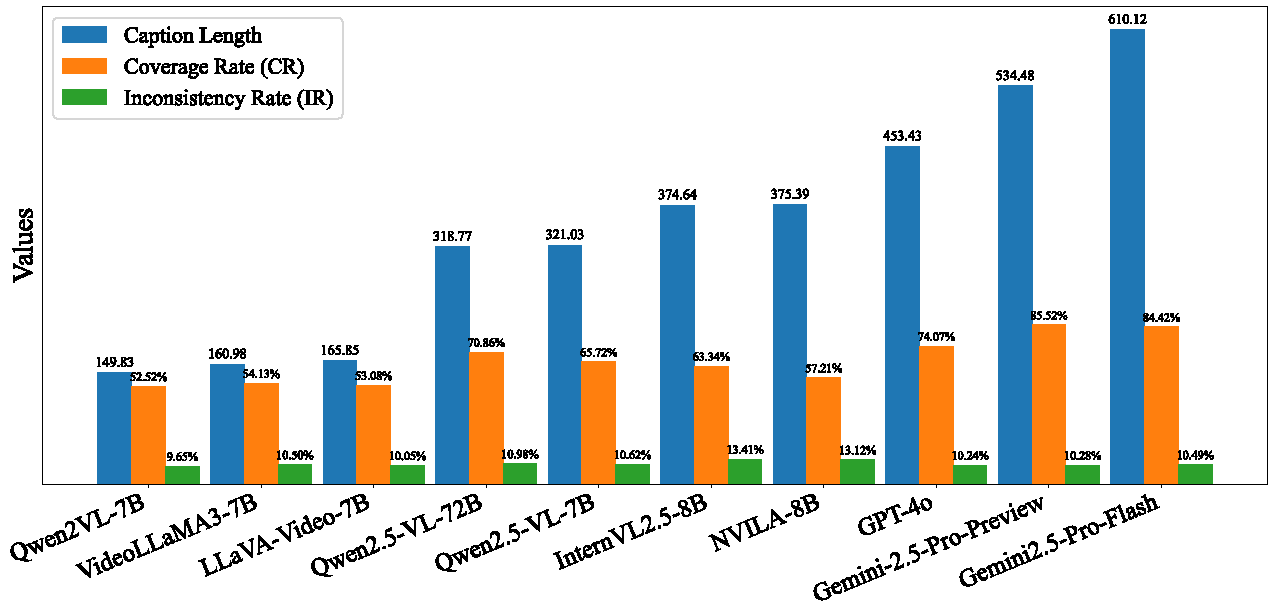
\includegraphics[width=0.9\linewidth]{imgs/comparison_chart_sorted_NEW22.pdf}
    \vspace{-0.5em}
	\caption{The relationship between CR, IR and caption length, where GPT-4.1 as a TextQA expert. Caption length is the number of words in the caption, not counting special symbols.}
	\label{fig:fig10}
	\end{minipage}%
\end{figure}

\begin{figure}[thbp]
	\begin{minipage}[t]{1.0\linewidth}
        \centering
	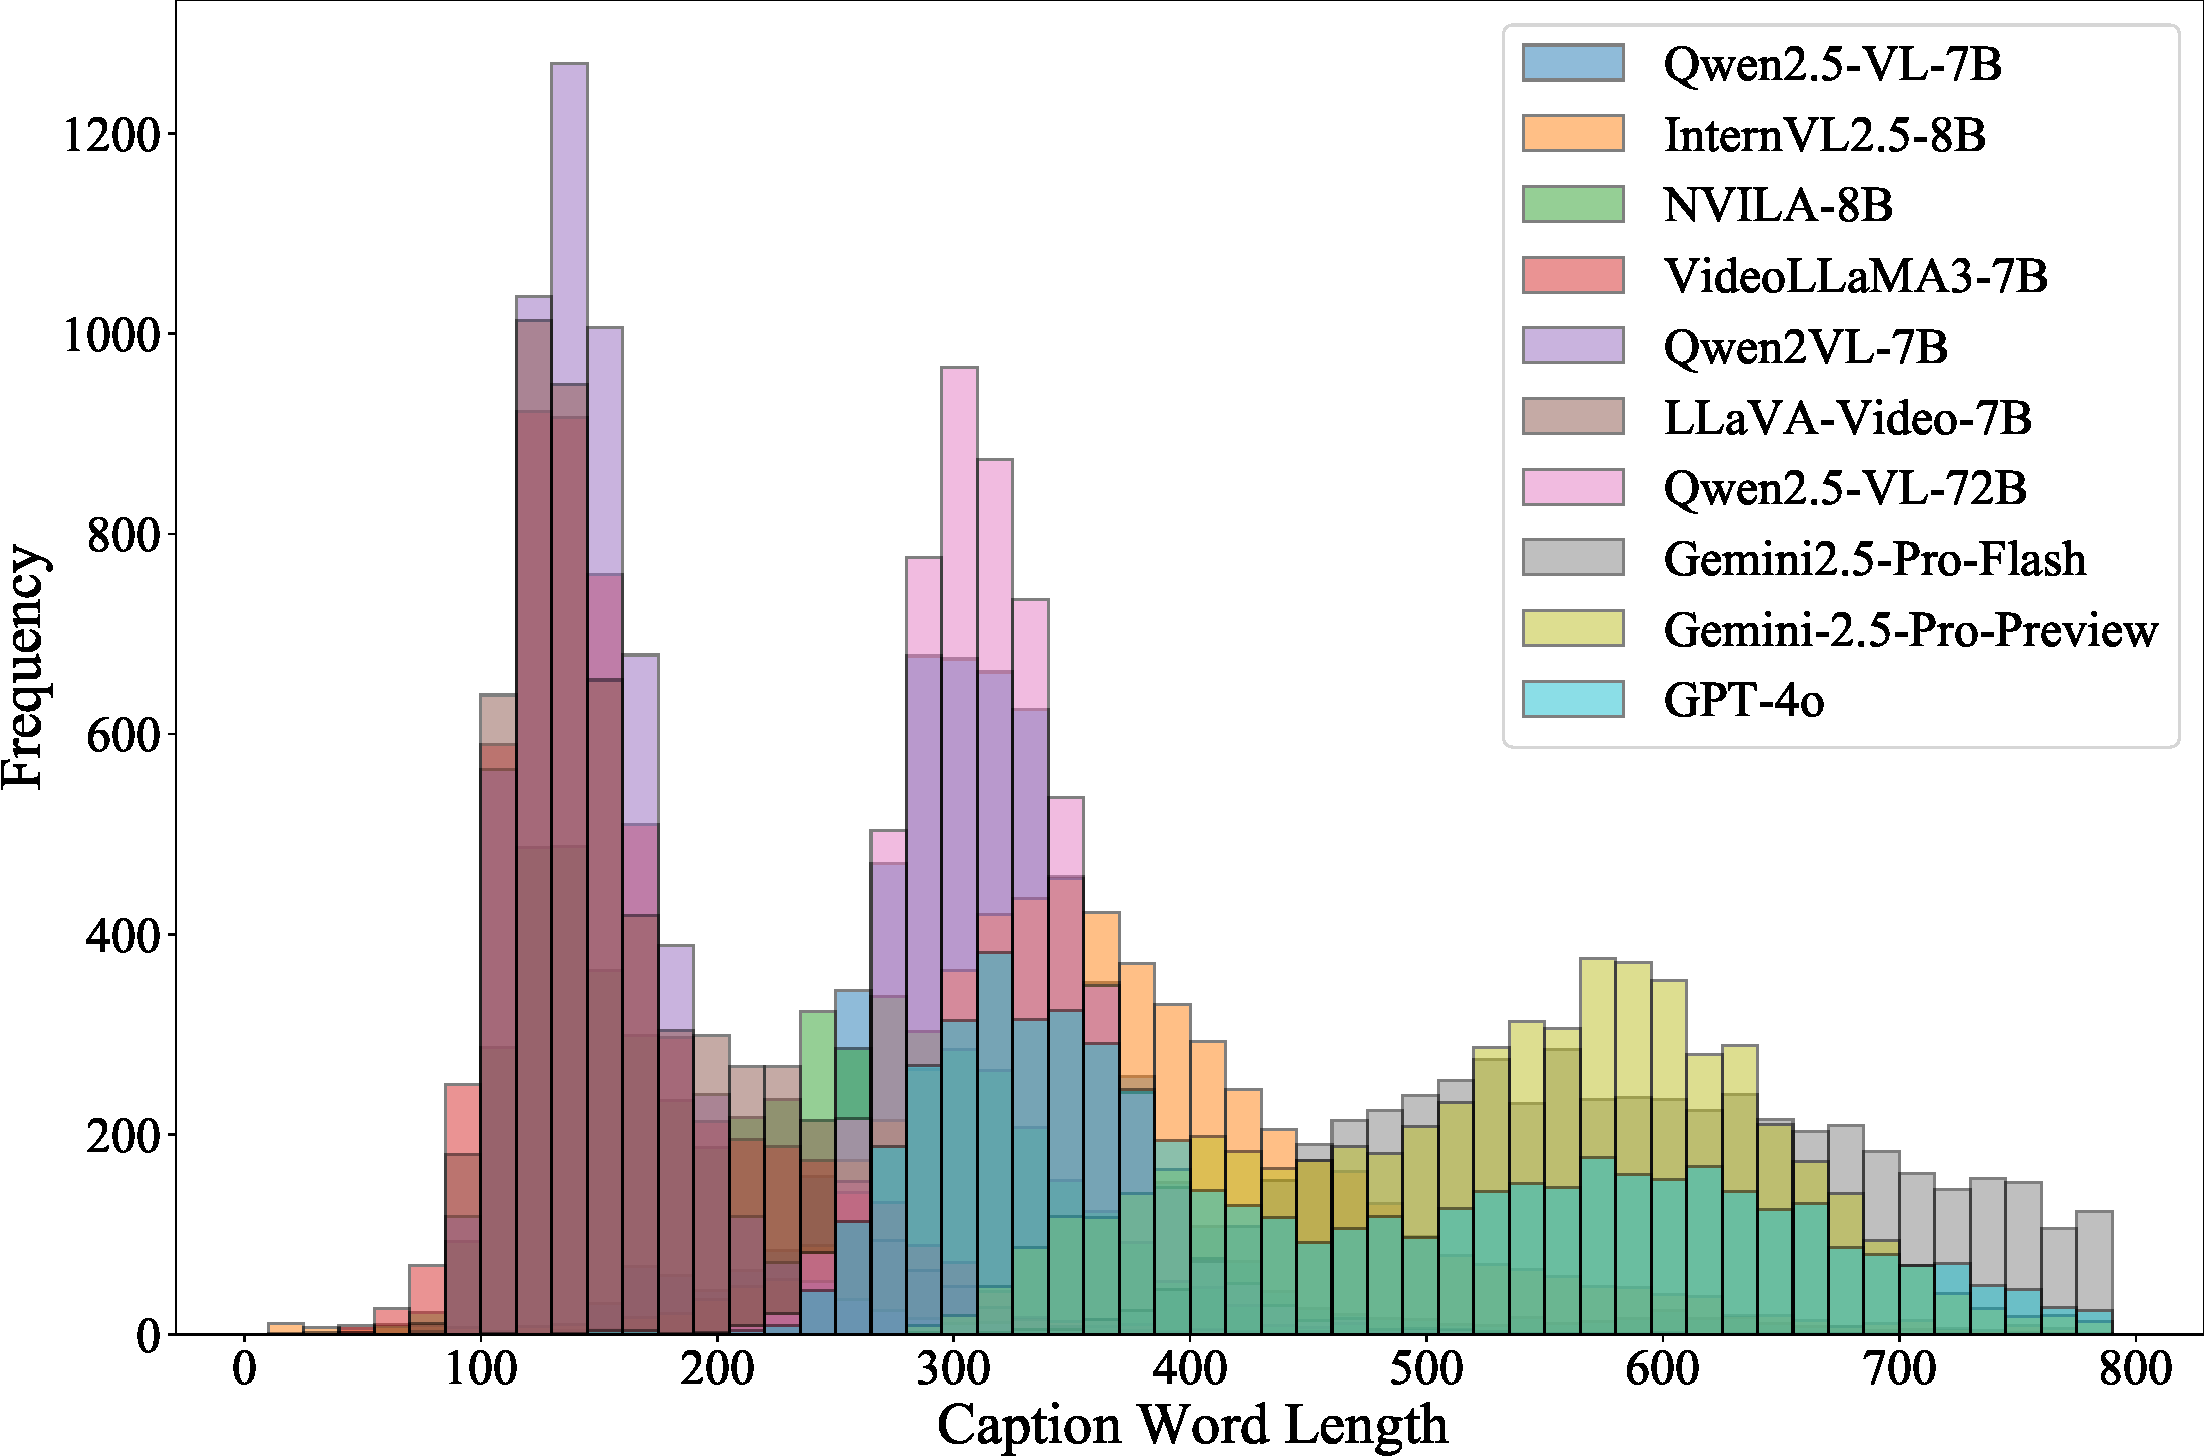
\includegraphics[width=0.9\linewidth]{imgs/word_length_distribution-all-3.pdf}
	\caption{Video caption word length distribution.}
	\label{fig:fig11}
	\end{minipage}%
\end{figure}


Table~\ref{tab:results_2} and Fig.~\ref{fig:fig9} presents the accuracy rate (AR), inconsistency rate (IR), and coverage rate (CR) of various VLM methods across multiple dimensions. Overall, Gemini-2.5-Pro-Preview achieves the best or second-best performance in nearly all categories. Notably, it attains the highest AR and CR in most dimensions, such as ``Background'' and  ``Camera Movement'', reaching 92.72\% and 92.09\%, respectively, which demonstrates its strong multimodal understanding capabilities. Meanwhile, its IR remains low, indicating good consistency in its responses. GPT-4o also shows competitive results in certain aspects (such as ``Entity Shape'' and ``Lighting''), but its overall performance is still slightly behind the Gemini series. In contrast, smaller models like LLaVA-Video-7B and Qwen2VL-7B lag significantly in all metrics, especially in complex scenarios and fine-grained attributes (\eg, ``Blur'' and ``Camera Movement''). In summary, as model scale and multimodal capabilities increase, VLMs exhibit substantial improvements in video understanding tasks, with Gemini-2.5-Pro-Preview currently demonstrating the best overall performance.



Fig.~\ref{fig:fig10} and Fig.~\ref{fig:fig11} compare the performance of various Vision-Language Models (VLMs) in terms of caption length, coverage rate (CR), and inconsistency rate (IR). As shown in Figure 1, advanced models such as Gemini-2.5-Pro-Flash, Gemini-2.5-Pro-Preview, and GPT-4o generate much longer captions and achieve higher coverage rates compared to earlier models like Qwen2VL-7B and VideoLLaMA3-7B. Despite the increase in caption length, the inconsistency rate remains low and stable across all models.

Fig.~\ref{fig:fig11} further illustrates the distribution of caption word lengths. Simpler models tend to produce shorter captions, while the more advanced models generate a wider range of longer captions. Overall, these results indicate that recent VLMs are capable of producing more detailed and comprehensive image descriptions without sacrificing consistency.

\subsection{The Impact of Evaluator Selection on the Results}\label{exp_app1}

\begin{table*}[htbp]
\renewcommand{\arraystretch}{0.6}
\caption{The accuracy (AR), inconsistency rate (IR), and coverage rate (CR) the captions of Gemini-2.5-Pro-Preview, GPT-4o and Qwen2.5-VL-72B, where we compare the results of Gemini-2.5-Pro-Preview, GPT-4o, and Manual comprehensive evaluation. The symbol ``$\uparrow$"  indicates that the larger the value, the better; The symbol ``$\downarrow$" indicates that the smaller the value, the better.}
\label{tab:results_3}
\resizebox{\textwidth}{!}{%
\begin{tabular}{@{}l|ccccccccc@{}}
\toprule
 \multirow{3}{*}{Methods}& \multicolumn{3}{c|}{Gemini-2.5-Pro-Preview}& \multicolumn{3}{c|}{GPT-4o}& \multicolumn{3}{c}{Qwen2.5-VL-72B}\\
 \cline{2-10} 
 & AR$\uparrow$ & IR$\downarrow$ &\multicolumn{1}{c|}{CR$\uparrow$}& AR$\uparrow$ & IR$\downarrow$ & \multicolumn{1}{c|}{CR$\uparrow$} & AR$\uparrow$ & IR$\downarrow$ & CR$\uparrow$  \\
 
 \midrule 
Manual &76.87&9.33&\multicolumn{1}{c|}{87.42} &65.47&13.33&\multicolumn{1}{c|}{74.22} &62.76&11.33&70.27\\
GPT-4o &76.73&10.28&\multicolumn{1}{c|}{85.52} &66.49&10.24&\multicolumn{1}{c|}{74.07} &63.08&10.98&70.86  \\ 
Gemini-2.5-Pro-Preview &73.88&14.62&\multicolumn{1}{c|}{86.52} &63.08&15.90&\multicolumn{1}{c|}{75.01} &61.20&16.02&72.87\\


\bottomrule
\end{tabular}%
}
\end{table*}

We randomly selected 100 samples from the dataset and evaluated the quality of video captions generated by different models (\eg, Gemini-2.5-Pro-Preview, GPT-4o and Qwen2.5-VL-72B) using three methods: manual evaluation, method~b, and method~c. The results are shown in Table~\ref{tab:results_3}. As observed, although there are some differences among the automatic evaluation methods, their results are generally consistent with the manual evaluation, and the performance gaps are not significant. This demonstrates that the proposed automatic evaluation process can effectively support the rapid assessment and optimization of video caption generation models.


\subsection{Limitations}\label{exp_app2}

A primary limitation of our proposed evaluation framework is its dependence on the capabilities of the large language model (LLM) employed as the evaluation expert. The use of different LLMs as evaluators may yield variations in the absolute quantitative scores assigned to model outputs. Nevertheless, as long as the same LLM is consistently used for evaluation and possesses sufficiently advanced capabilities (\eg, GPT-4.1 or Gemini 2.5), it can reliably distinguish the relative quality of video captions generated by different models. In general, the reliability of the evaluation results improves with the strength of the LLM serving as the evaluator. We anticipate that, with the ongoing rapid progress in LLM development, the accuracy and robustness of our automatic evaluation framework will continue to improve, further enhancing its utility for video captioning assessment.


\iftoggle{isSubmission}{
  \section*{NeurIPS Paper Checklist}

\begin{enumerate}

\item {\bf Claims}
    \item[] Question: Do the main claims made in the abstract and introduction accurately reflect the paper's contributions and scope?
    \item[] Answer: \answerYes{} % Replace by \answerYes{}, \answerNo{}, or \answerNA{}.
    \item[] Justification: The main claims in the abstract and introduction are consistent with the paper's actual contributions and scope.
    \item[] Guidelines:
    \begin{itemize}
        \item The answer NA means that the abstract and introduction do not include the claims made in the paper.
        \item The abstract and/or introduction should clearly state the claims made, including the contributions made in the paper and important assumptions and limitations. A No or NA answer to this question will not be perceived well by the reviewers. 
        \item The claims made should match theoretical and experimental results, and reflect how much the results can be expected to generalize to other settings. 
        \item It is fine to include aspirational goals as motivation as long as it is clear that these goals are not attained by the paper. 
    \end{itemize}

\item {\bf Limitations}
    \item[] Question: Does the paper discuss the limitations of the work performed by the authors?
    \item[] Answer: \answerYes{} % Replace by \answerYes{}, \answerNo{}, or \answerNA{}.
    \item[] Justification: The paper includes a dedicated section (A.3 Limitations) discussing the limitations of the work.
    \item[] Guidelines:
    \begin{itemize}
        \item The answer NA means that the paper has no limitation while the answer No means that the paper has limitations, but those are not discussed in the paper. 
        \item The authors are encouraged to create a separate "Limitations" section in their paper.
        \item The paper should point out any strong assumptions and how robust the results are to violations of these assumptions (e.g., independence assumptions, noiseless settings, model well-specification, asymptotic approximations only holding locally). The authors should reflect on how these assumptions might be violated in practice and what the implications would be.
        \item The authors should reflect on the scope of the claims made, e.g., if the approach was only tested on a few datasets or with a few runs. In general, empirical results often depend on implicit assumptions, which should be articulated.
        \item The authors should reflect on the factors that influence the performance of the approach. For example, a facial recognition algorithm may perform poorly when image resolution is low or images are taken in low lighting. Or a speech-to-text system might not be used reliably to provide closed captions for online lectures because it fails to handle technical jargon.
        \item The authors should discuss the computational efficiency of the proposed algorithms and how they scale with dataset size.
        \item If applicable, the authors should discuss possible limitations of their approach to address problems of privacy and fairness.
        \item While the authors might fear that complete honesty about limitations might be used by reviewers as grounds for rejection, a worse outcome might be that reviewers discover limitations that aren't acknowledged in the paper. The authors should use their best judgment and recognize that individual actions in favor of transparency play an important role in developing norms that preserve the integrity of the community. Reviewers will be specifically instructed to not penalize honesty concerning limitations.
    \end{itemize}

\item {\bf Theory assumptions and proofs}
    \item[] Question: For each theoretical result, does the paper provide the full set of assumptions and a complete (and correct) proof?
    \item[] Answer: \answerNo{} % Replace by \answerYes{}, \answerNo{}, or \answerNA{}.
    \item[] Justification: In this paper, we introduce a dataset for assessing the quality of video captions. Notably, our approach does not depend on theoretical assumptions, nor does it require formal theoretical proofs.
    \item[] Guidelines:
    \begin{itemize}
        \item The answer NA means that the paper does not include theoretical results. 
        \item All the theorems, formulas, and proofs in the paper should be numbered and cross-referenced.
        \item All assumptions should be clearly stated or referenced in the statement of any theorems.
        \item The proofs can either appear in the main paper or the supplemental material, but if they appear in the supplemental material, the authors are encouraged to provide a short proof sketch to provide intuition. 
        \item Inversely, any informal proof provided in the core of the paper should be complemented by formal proofs provided in appendix or supplemental material.
        \item Theorems and Lemmas that the proof relies upon should be properly referenced. 
    \end{itemize}

    \item {\bf Experimental result reproducibility}
    \item[] Question: Does the paper fully disclose all the information needed to reproduce the main experimental results of the paper to the extent that it affects the main claims and/or conclusions of the paper (regardless of whether the code and data are provided or not)?
    \item[] Answer: \answerYes{} % Replace by \answerYes{}, \answerNo{}, or \answerNA{}.
    \item[] Justification: All data used in this study are made available, including the original videos, the annotated QA-pair files, the video captions generated by the VLMs described in the paper, and the corresponding evaluation results produced by the expert evaluators.
    \item[] Guidelines:
    \begin{itemize}
        \item The answer NA means that the paper does not include experiments.
        \item If the paper includes experiments, a No answer to this question will not be perceived well by the reviewers: Making the paper reproducible is important, regardless of whether the code and data are provided or not.
        \item If the contribution is a dataset and/or model, the authors should describe the steps taken to make their results reproducible or verifiable. 
        \item Depending on the contribution, reproducibility can be accomplished in various ways. For example, if the contribution is a novel architecture, describing the architecture fully might suffice, or if the contribution is a specific model and empirical evaluation, it may be necessary to either make it possible for others to replicate the model with the same dataset, or provide access to the model. In general. releasing code and data is often one good way to accomplish this, but reproducibility can also be provided via detailed instructions for how to replicate the results, access to a hosted model (e.g., in the case of a large language model), releasing of a model checkpoint, or other means that are appropriate to the research performed.
        \item While NeurIPS does not require releasing code, the conference does require all submissions to provide some reasonable avenue for reproducibility, which may depend on the nature of the contribution. For example
        \begin{enumerate}
            \item If the contribution is primarily a new algorithm, the paper should make it clear how to reproduce that algorithm.
            \item If the contribution is primarily a new model architecture, the paper should describe the architecture clearly and fully.
            \item If the contribution is a new model (e.g., a large language model), then there should either be a way to access this model for reproducing the results or a way to reproduce the model (e.g., with an open-source dataset or instructions for how to construct the dataset).
            \item We recognize that reproducibility may be tricky in some cases, in which case authors are welcome to describe the particular way they provide for reproducibility. In the case of closed-source models, it may be that access to the model is limited in some way (e.g., to registered users), but it should be possible for other researchers to have some path to reproducing or verifying the results.
        \end{enumerate}
    \end{itemize}


\item {\bf Open access to data and code}
    \item[] Question: Does the paper provide open access to the data and code, with sufficient instructions to faithfully reproduce the main experimental results, as described in supplemental material?
    \item[] Answer: \answerYes{} % Replace by \answerYes{}, \answerNo{}, or \answerNA{}.
    \item[] Justification: All data utilized in this study are made publicly available, including the original videos, annotated QA-pair files, video captions generated by the VLMs discussed in the manuscript, and the corresponding evaluation results provided by expert evaluators. Furthermore, we release the evaluation scripts as well as the prompts employed for video caption generation, to facilitate reproducibility and further research.
    \item[] Guidelines:
    \begin{itemize}
        \item The answer NA means that paper does not include experiments requiring code.
        \item Please see the NeurIPS code and data submission guidelines (\url{https://nips.cc/public/guides/CodeSubmissionPolicy}) for more details.
        \item While we encourage the release of code and data, we understand that this might not be possible, so “No” is an acceptable answer. Papers cannot be rejected simply for not including code, unless this is central to the contribution (e.g., for a new open-source benchmark).
        \item The instructions should contain the exact command and environment needed to run to reproduce the results. See the NeurIPS code and data submission guidelines (\url{https://nips.cc/public/guides/CodeSubmissionPolicy}) for more details.
        \item The authors should provide instructions on data access and preparation, including how to access the raw data, preprocessed data, intermediate data, and generated data, etc.
        \item The authors should provide scripts to reproduce all experimental results for the new proposed method and baselines. If only a subset of experiments are reproducible, they should state which ones are omitted from the script and why.
        \item At submission time, to preserve anonymity, the authors should release anonymized versions (if applicable).
        \item Providing as much information as possible in supplemental material (appended to the paper) is recommended, but including URLs to data and code is permitted.
    \end{itemize}


\item {\bf Experimental setting/details}
    \item[] Question: Does the paper specify all the training and test details (e.g., data splits, hyperparameters, how they were chosen, type of optimizer, etc.) necessary to understand the results?
    \item[] Answer: \answerYes{} % Replace by \answerYes{}, \answerNo{}, or \answerNA{}.
    \item[] Justification: These details can be found in the experimental section of the paper and in the supplementary materials.
    \item[] Guidelines:
    \begin{itemize}
        \item The answer NA means that the paper does not include experiments.
        \item The experimental setting should be presented in the core of the paper to a level of detail that is necessary to appreciate the results and make sense of them.
        \item The full details can be provided either with the code, in appendix, or as supplemental material.
    \end{itemize}

\item {\bf Experiment statistical significance}
    \item[] Question: Does the paper report error bars suitably and correctly defined or other appropriate information about the statistical significance of the experiments?
    \item[] Answer: \answerYes{} % Replace by \answerYes{}, \answerNo{}, or \answerNA{}.
    \item[] Justification: To analyze the variability and potential sources of error in the evaluation results, we compared the assessments provided by different expert evaluators.
    \item[] Guidelines:
    \begin{itemize}
        \item The answer NA means that the paper does not include experiments.
        \item The authors should answer "Yes" if the results are accompanied by error bars, confidence intervals, or statistical significance tests, at least for the experiments that support the main claims of the paper.
        \item The factors of variability that the error bars are capturing should be clearly stated (for example, train/test split, initialization, random drawing of some parameter, or overall run with given experimental conditions).
        \item The method for calculating the error bars should be explained (closed form formula, call to a library function, bootstrap, etc.)
        \item The assumptions made should be given (e.g., Normally distributed errors).
        \item It should be clear whether the error bar is the standard deviation or the standard error of the mean.
        \item It is OK to report 1-sigma error bars, but one should state it. The authors should preferably report a 2-sigma error bar than state that they have a 96\% CI, if the hypothesis of Normality of errors is not verified.
        \item For asymmetric distributions, the authors should be careful not to show in tables or figures symmetric error bars that would yield results that are out of range (e.g. negative error rates).
        \item If error bars are reported in tables or plots, The authors should explain in the text how they were calculated and reference the corresponding figures or tables in the text.
    \end{itemize}

\item {\bf Experiments compute resources}
    \item[] Question: For each experiment, does the paper provide sufficient information on the computer resources (type of compute workers, memory, time of execution) needed to reproduce the experiments?
    \item[] Answer: \answerNo{} % Replace by \answerYes{}, \answerNo{}, or \answerNA{}.
    \item[] Justification: As our primary contribution is to provide a benchmark dataset for video caption quality assessment, information about computational resources (\eg, worker type, memory, execution time) is not the focus of our work, since we do not aim to optimize model efficiency. Our evaluations are performed using the currently available VLMs, and details regarding resource usage can be found in the respective technical reports of these models.
    \item[] Guidelines:
    \begin{itemize}
        \item The answer NA means that the paper does not include experiments.
        \item The paper should indicate the type of compute workers CPU or GPU, internal cluster, or cloud provider, including relevant memory and storage.
        \item The paper should provide the amount of compute required for each of the individual experimental runs as well as estimate the total compute. 
        \item The paper should disclose whether the full research project required more compute than the experiments reported in the paper (e.g., preliminary or failed experiments that didn't make it into the paper). 
    \end{itemize}
    
\item {\bf Code of ethics}
    \item[] Question: Does the research conducted in the paper conform, in every respect, with the NeurIPS Code of Ethics \url{https://neurips.cc/public/EthicsGuidelines}?
    \item[] Answer: \answerYes{} % Replace by \answerYes{}, \answerNo{}, or \answerNA{}.
    \item[] Justification: the research conducted in the paper fully conforms to the NeurIPS Code of Ethics in every respect.
    \item[] Guidelines:
    \begin{itemize}
        \item The answer NA means that the authors have not reviewed the NeurIPS Code of Ethics.
        \item If the authors answer No, they should explain the special circumstances that require a deviation from the Code of Ethics.
        \item The authors should make sure to preserve anonymity (e.g., if there is a special consideration due to laws or regulations in their jurisdiction).
    \end{itemize}


\item {\bf Broader impacts}
    \item[] Question: Does the paper discuss both potential positive societal impacts and negative societal impacts of the work performed?
    \item[] Answer: \answerYes{} % Replace by \answerYes{}, \answerNo{}, or \answerNA{}.
    \item[] Justification: This issue has been discussed in the experimental section of the paper.
    \item[] Guidelines:
    \begin{itemize}
        \item The answer NA means that there is no societal impact of the work performed.
        \item If the authors answer NA or No, they should explain why their work has no societal impact or why the paper does not address societal impact.
        \item Examples of negative societal impacts include potential malicious or unintended uses (e.g., disinformation, generating fake profiles, surveillance), fairness considerations (e.g., deployment of technologies that could make decisions that unfairly impact specific groups), privacy considerations, and security considerations.
        \item The conference expects that many papers will be foundational research and not tied to particular applications, let alone deployments. However, if there is a direct path to any negative applications, the authors should point it out. For example, it is legitimate to point out that an improvement in the quality of generative models could be used to generate deepfakes for disinformation. On the other hand, it is not needed to point out that a generic algorithm for optimizing neural networks could enable people to train models that generate Deepfakes faster.
        \item The authors should consider possible harms that could arise when the technology is being used as intended and functioning correctly, harms that could arise when the technology is being used as intended but gives incorrect results, and harms following from (intentional or unintentional) misuse of the technology.
        \item If there are negative societal impacts, the authors could also discuss possible mitigation strategies (e.g., gated release of models, providing defenses in addition to attacks, mechanisms for monitoring misuse, mechanisms to monitor how a system learns from feedback over time, improving the efficiency and accessibility of ML).
    \end{itemize}
    
\item {\bf Safeguards}
    \item[] Question: Does the paper describe safeguards that have been put in place for responsible release of data or models that have a high risk for misuse (e.g., pretrained language models, image generators, or scraped datasets)?
    \item[] Answer: \answerNo{} % Replace by \answerYes{}, \answerNo{}, or \answerNA{}.
    \item[] Justification: This paper does not involve the release of any data or models that pose a high risk for misuse, such as pretrained language models, image generators, or scraped datasets.
    \item[] Guidelines:
    \begin{itemize}
        \item The answer NA means that the paper poses no such risks.
        \item Released models that have a high risk for misuse or dual-use should be released with necessary safeguards to allow for controlled use of the model, for example by requiring that users adhere to usage guidelines or restrictions to access the model or implementing safety filters. 
        \item Datasets that have been scraped from the Internet could pose safety risks. The authors should describe how they avoided releasing unsafe images.
        \item We recognize that providing effective safeguards is challenging, and many papers do not require this, but we encourage authors to take this into account and make a best faith effort.
    \end{itemize}

\item {\bf Licenses for existing assets}
    \item[] Question: Are the creators or original owners of assets (e.g., code, data, models), used in the paper, properly credited and are the license and terms of use explicitly mentioned and properly respected?
    \item[] Answer: \answerYes{} % Replace by \answerYes{}, \answerNo{}, or \answerNA{}.
    \item[] Justification: All assets used in this paper are properly credited. The data used in our experiments are obtained from publicly available open-source datasets, and we have explicitly cited the original sources in the paper. We have carefully reviewed and respected the licenses and terms of use associated with these datasets.
    \item[] Guidelines:
    \begin{itemize}
        \item The answer NA means that the paper does not use existing assets.
        \item The authors should cite the original paper that produced the code package or dataset.
        \item The authors should state which version of the asset is used and, if possible, include a URL.
        \item The name of the license (e.g., CC-BY 4.0) should be included for each asset.
        \item For scraped data from a particular source (e.g., website), the copyright and terms of service of that source should be provided.
        \item If assets are released, the license, copyright information, and terms of use in the package should be provided. For popular datasets, \url{paperswithcode.com/datasets} has curated licenses for some datasets. Their licensing guide can help determine the license of a dataset.
        \item For existing datasets that are re-packaged, both the original license and the license of the derived asset (if it has changed) should be provided.
        \item If this information is not available online, the authors are encouraged to reach out to the asset's creators.
    \end{itemize}

\item {\bf New assets}
    \item[] Question: Are new assets introduced in the paper well documented and is the documentation provided alongside the assets?
    \item[] Answer: \answerYes{} % Replace by \answerYes{}, \answerNo{}, or \answerNA{}.
    \item[] Justification: This paper presents a new dataset, which is openly accessible via Hugging Face and GitHub. We have included thorough documentation and detailed descriptions to ensure transparency and ease of use for other researchers.
    \item[] Guidelines:
    \begin{itemize}
        \item The answer NA means that the paper does not release new assets.
        \item Researchers should communicate the details of the dataset/code/model as part of their submissions via structured templates. This includes details about training, license, limitations, etc. 
        \item The paper should discuss whether and how consent was obtained from people whose asset is used.
        \item At submission time, remember to anonymize your assets (if applicable). You can either create an anonymized URL or include an anonymized zip file.
    \end{itemize}

\item {\bf Crowdsourcing and research with human subjects}
    \item[] Question: For crowdsourcing experiments and research with human subjects, does the paper include the full text of instructions given to participants and screenshots, if applicable, as well as details about compensation (if any)? 
    \item[] Answer: \answerNo{} % Replace by \answerYes{}, \answerNo{}, or \answerNA{}.
    \item[] Justification: this paper does not involve any crowdsourcing experiments or research with human subjects.
    \item[] Guidelines:
    \begin{itemize}
        \item The answer NA means that the paper does not involve crowdsourcing nor research with human subjects.
        \item Including this information in the supplemental material is fine, but if the main contribution of the paper involves human subjects, then as much detail as possible should be included in the main paper. 
        \item According to the NeurIPS Code of Ethics, workers involved in data collection, curation, or other labor should be paid at least the minimum wage in the country of the data collector. 
    \end{itemize}

\item {\bf Institutional review board (IRB) approvals or equivalent for research with human subjects}
    \item[] Question: Does the paper describe potential risks incurred by study participants, whether such risks were disclosed to the subjects, and whether Institutional Review Board (IRB) approvals (or an equivalent approval/review based on the requirements of your country or institution) were obtained?
    \item[] Answer: \answerNo{} % Replace by \answerYes{}, \answerNo{}, or \answerNA{}.
    \item[] Justification: This paper does not involve research with human subjects, and therefore IRB approval or equivalent review was not required.
    \item[] Guidelines:
    \begin{itemize}
        \item The answer NA means that the paper does not involve crowdsourcing nor research with human subjects.
        \item Depending on the country in which research is conducted, IRB approval (or equivalent) may be required for any human subjects research. If you obtained IRB approval, you should clearly state this in the paper. 
        \item We recognize that the procedures for this may vary significantly between institutions and locations, and we expect authors to adhere to the NeurIPS Code of Ethics and the guidelines for their institution. 
        \item For initial submissions, do not include any information that would break anonymity (if applicable), such as the institution conducting the review.
    \end{itemize}

\item {\bf Declaration of LLM usage}
    \item[] Question: Does the paper describe the usage of LLMs if it is an important, original, or non-standard component of the core methods in this research? Note that if the LLM is used only for writing, editing, or formatting purposes and does not impact the core methodology, scientific rigorousness, or originality of the research, declaration is not required.
    %this research? 
    \item[] Answer: \answerYes{} % Replace by \answerYes{}, \answerNo{}, or \answerNA{}.
    \item[] Justification: The paper details the use of LLMs as a key and original part of the research methodology. In particular, LLMs are utilized as evaluation experts and actively participate in the process of generating video captions.
    \item[] Guidelines:
    \begin{itemize}
        \item The answer NA means that the core method development in this research does not involve LLMs as any important, original, or non-standard components.
        \item Please refer to our LLM policy (\url{https://neurips.cc/Conferences/2025/LLM}) for what should or should not be described.
    \end{itemize}

\end{enumerate}
}

\end{document}